%MEGA MAN X2.TEX

\textit{Mega Man X2} is the direct sequel of the first \textit{Mega Man X} game, released in Japan on December 16, 1994, and in North America and PAL regions in 1995, one year after the release of the first game. The game features the same gameplay and graphics of its predecessor, but  Capcom included the Cx4 enhancement chip inside the cartridge, which allowed for the usage of 3D wireframe effects whose the development team was instructed to utilize for as much as possible when working on the game~\cite{wiki:MMX2}. The game, however, also had an extensive script localization in the American version which resulted in the removal of important detail and links in favor of a easier to follow,yet incomplete, script (such as changing all occurrences of X's name with \textit{Mega Man X}). In order to avoid confusion, in this chapter all plot-related events will come from direct translations from the Japanese game script (found in \cite{wordpress:X2_japanese_script} and \cite{gamesfaq:X2_japanese_script}).

\section{Main plot}
Six months later Sigma's defeat by X, mavericks are still posing a threat to mankind and reploids. Maverick Haunters are still fighting against them to restore peace, but the heavy losses undergone during the first revolution has reduced the number of available haunters to a quarter of their original value~\cite{Xcoll1:Manual_X2}. Furthermore in later periods maverick attack have been increasing in number and many Maverick Haunters bases have been attacked and destroyed, despite the original number of reploids joining Sigma wasn't very high. What makes the situation even worse is that by analyzing defeated mavericks, scientists have found a special chip bearing Sigma's insignia, installed at the moment of their creation responsible for them going maverick. After some researches, maverick haunters manage to locate the factory where these mavericks are created and X, alongside the 17th Unit, begins its attack to the facility.

It is during this operation that Mega Man X2 starts: after an harsh fight outside the facility, X manages to enter and destroy it, but only after having dealt with one of the giant mechaniloid CF-0 produced in the factory. After the fight the scene moves away from X, revealing three figures in the shadow, observing X's movement on a monitor and commenting on how he could pose a threat to their plans. Although they do not seem to fear him they recognize his strength and the fact that he could interfere in their plans, for which they're in hurry, and decide to leave him fight with their eight maverick subordinates to gather time and complete their scheme.

X, however, prove himself to be far superior respect the three figure's expectations, disposing of mavericks at a faster rate than imagined. These leads the three figures to come out from the shadows and face X directly, both slow down X and attempting to eliminate him by themselves. The three contact than the Maverick Haunter headquarters and present themselves: they're Agile, Serges and Violen leaders of a group called the ``X-Haunters'' (\textit{``Counter-Haunter''} in the Japanese version) which act has a counterpart to the Maverick Haunters and aims to destroy them. The three pose a challenge X : if he manages to locate and fight all of them in a one-vs-one fight, for each of them X defeats he will receive one of Zero's body part they had previously retrieved and repaired. These, together with Zero's control parts recovered and preserved inside the M.H. headquarter, could allow him to resurrect his friend. For here the story can take two paths, depending weather the player manages to locate and defeat all the X-Haunters or not:
If X gather all Zero's parts Dr.~Cain will begin his reparation, and in the meanwhile he will also locate the X-Haunters fortress; on the other hand, should X miss at least one of them, they will storm Dr.~Cain's laboratory and steal all Zero's component, control circuit included, to revive him as a Maverick, but also leaving a trace pointing to their headquarter, which in both case results to be located in the north pole.

Once reached the X-Haunter fortress, X infiltrates inside and fight once more against the X-Haunters, only this time their objective is to effectively dispose of him and not to slow down. This translates in them recurring to their full power and all means to take down X: Violen challenges X as Neo Violen, a more powerful form of him, Serges tries to stop him by recurring to his Serges Tank and finally Agile by using the Agile Flyer; however none of them succeed in the plan and are all defeated by X. Unluckily for X though, X-Haunters plan was in the end completed as a reborn Sigma contact X while the fortress he is in starts exploding, and challenges him to a fight in the Central computer, a location already visited by X while facing mavericks sent by the X-Haunters. Once X reaches the location, two events can occur based on the outcome of Zero's quest.

Shouldn't X have recover all Zero's part, allowing the X-Haunters to stole all the remaining one, he will find Sigma, with his new body, alongside a repaired Zero which however doesn't show any sign of consciousness, as he attacks X as soon as Sigma orders him to do it. Only after being defeated by X Zero regain his consciousness, as he apologize to X for all the trouble he has caused and decides to help X opening a passage for him to reach Sigma.

If instead X managed to recover all Zero's parts when reaching the Central Computer he will find instead Sigma alongside a black replica of Zero, which Sigma intend to use against X. Luckily the real Zero appear, easily destroying his replica and leaving Sigma surprised in finding out Zero decided to size with X. After this dialogue Sigma retreats, but Zero opens up a passage for X to chase him down.

Whatever of the two previous events happen, in the end X will always reach the final confrontation with Sigma, reborn in a new body and ready to face X once more. As in the previous game, however, X manages to destroy Sigma's new body but this time only to reveal Sigma's true form: the Sigma virus. Sigma appears in fact not anymore as an actual reploid, but rather as a materialized virus with a consciousness. After a long battle X finally manages to defeat Sigma again, which disappears but before making his final warning. This time however, instead of blaming X for the failure of his plans, Sigma warns X that he will always manage to match his power, whatever the level his. Nevertheless, one thing seems to bother Sigma while disappearing, this being Zero siding with X. Sigma, in fact, was sure beyond any limit that Zero would have followed him, almost as it was his destiny.

After Sigma's defeat, X and Zero reunite together near a seaside. Here X ponders again on the reason of his fight, on why he has such incredible power within him and, more importantly, if he will ever been capable of admiring realized the dream of a world where humans and reploids coexists and that Dr.~Light dreamed of.

\section{Main Characters}

\subsection{X}
X (see also chap.~[\ref{char:X}])  is Dr.~Light's last creation and the basis on which Dr.~Cain developed all reploids, although X's technology cannot be fully understand even with the knowledge of the time. When Sigma began his revolution against humanity X stood up and fought him, putting an halt to Sigma's plans and bringing peace to the world. Thanks to this, X was promoted leader of the 17th Elite Unit, which he belongs to and was previously lead by Sigma himself and Zero, a close friend of X which sacrificed himself to save him, but his haunter rank have remained unchanged although some people have started noticing that X's hidden potential could even surpass the abilities of SA-ranked haunters.

Despite his incredible power, X remains a kindhearted person which refuse to believe violence is the only solution to the maverick problems, and the turmoil caused by his kind spirit and the need to fight to protect innocent is something very few people understand\cite{Xcoll1:Manual_X2}.

\subsection{Zero}
Zero (chap.~[\ref{char:Zero}]) was an SA-ranked Maverick haunter under the 17th Elite unit and was X's best friend as well as only one of few people who could truly understands X's feelings. During Sigma' war he was appointed leader of the Maverick Haunters and lead the others against Sigma. However near the end of the conflict Zero was forced to detonate his energy core to protect his friend X, dying in the process. Luckily his control chip remained intact and was brought to the Maverick Haunters headquarters where they reside during the event of this game.

Similar to X, however, Zero's body is far too complex to be repaired even by a scientist of Dr.~Cain's level, but not for X-Haunter's scientist Serges, who not only manages to repair Zero's body but even to upgrade it in order to revive him as a Maverick\cite{wayback:X2_resources} (even succeeding depending on which ending the player achieve). Whether to be Serges or Dr.~Cain (with Serges's rebuilt parts) to rebuild him, Zero makes his return at the end of the game, where he either challenges X or destroy his copy, and opens the to Sigma for X. He is later seen during the end, gazing at the sea near his friend.


\subsection{Dr.~Cain}
Dr.~Cain (chap.~[\ref{char:Cain}]) is the greatest expert in robotics of the 22$^nd$ century\cite{Xcoll1:Manual_X2}. By using Dr.~Light's schematics and X's help, he solely managed to transform robots of his times, by introducing reploids, robot perfectly capable of think and act autonomously as well as showing emotions. This, however, also lead to the appear of mavericks, not last Sigma which, by chance, was Dr.~Cain greatest creation. In the present Dr.~Cain act is also the founder of Maverick Haunters, also covering a position on its high vertex as well as playing a supportive role in the Maverick haunt, as the X2 games show. Here, in fact, Dr.~Cain coordinate X's operation from remote, locating in the end the X-Haunter's base for the final attacks. He also works to restore and repair Zero, but only when provided with all already-restored parts X recovers from all the X-Haunters.

\subsection{X-Haunters}
After Sigma's defeat by the hand of X, it was believed mavericks attacks would have cease, as there was no leader to command them. But this was not the case. Although at first the loss of their leader may have lead the maverick army to a series of losses against the more organized, even if weakened Maverick Haunters, not so much time had to pass before a new head would appear to lead the rebellion. Only this time instead of a single one, three reploids took charge of the army: a group called the X-Haunters.

Composed by three incredibly strong reploids, Agile, Serges and Violen, this group takes lead of Sigma's army, and re-organized it in order to bring on Sigma's plan from where it stopped. The first step consists in the creation of more maverick troops in order to reinforce the army. To do so a reploid factory is conquered and altered in order to implant special chips inside produced reploids to brainwash them into loyal maverick soldiers. Furthermore inside the factory giant reploids CF-0 are also build to increase even more their military potential.

The second, and more important step, in X-Haunters plans, is the revive of both Zero and Sigma. This plan, however, requires a large amount of time to be completed, as only Serges is the one capable of building a new body for Sigma and repair Zero's parts they recovered. Beside time, the other limiting factor to the plan is the missing of Zero's own control circuit, the only component saved by Maverick haunters and now stored in their headquarters. To gain time to complete their project, the three decides to deploy the eight SA-ranked maverick they have to hit strategical objectives and slow down haunter's operations. They however underestimate X's strength, as he disposes of deployed maverick at a much faster rate their plan proceed, which force them to intervene in first person and, more importantly, to use Zero's part they restored  as prize to force X into a fight, with the risk of loosing a key factor of their plan. Depending on how the game proceed, they can either be all defeated, which leads them to retreat into their fortress and hurry to complete their plan by creating a fake Zero replica, or survive the fight with X, giving them the chance to attack the Haunter's headquarter while X isn't there and stole all Zero's components, to fully resurrect him as a maverick, but also leaving a trace for X to follow them to their hideout.

In both cases, X manages to find the X-haunters headquarters and begins his attack. To stop him, the three decide to fight him each one on their own and using all their available equipment to surpass him in strength. However none of the three succeeds, as all of them in the end are defeated and destroyed by X.


\section{Game Mechanics}
Being a direct sequel of \textit{Mega Man X}, \textit{Mega Man X2} reuses almost every game mechanics present in the first title, while also bringing some new feature to the gameplay:
\begin{itemize}
	\item Dashing: X now has the ability to dash from the start. However this ability can be further enhanced, allowing for air-dashing.
	\item Stage Interactions: stages now no longer interact between them, hence beating a level now doesn't grant any vantages in another one.
	\item ``Refill'' rooms: some stages have special rooms which at first present themselves as empty room, but if X release a charged Silk Shot inside them it will attract various health and energy capsule for X to collect, without a limit to how many times this operation can be done.
	\item X-Haunter challenges: Once the second boss is defeated, the three X-Haunters will begin appearing inside remaining levels. X-haunters movements can be seen in the map screen as soon as the player return to it, where the player will see the remaining haunters teleporting from one stage to another. Once inside a stage the X-haunter can be challenged inside a secret room X can met while traveling the level, but which normally are inaccessible. For each haunter defeated X will receive a Zero part to resurrect his friend, meanwhile skipping the fight will cause the X-haunter to flee forever, losing the chance to get the part for good. Finally should the player get a game-over, or enter and exit an already-beaten level, it will trigger X-haunters movement across remaining levels.
	\item Ride Chaser %%
	\item New Ride Armor
\end{itemize}

\section{Weapons}\label{X2:sub_weapon}
Here are now listed all sub-weapons available inside \textit{Mega Man X2}~\cite{wiki:X_weapons}

\subsection{
\includegraphics[width=12px, height=10px]{figures/X2/weapons/C_haunter.png} Crystal Haunter}\label{Crystal_haunter}
Crystal Haunter shots a glob of liquid which crystallize small enemies that comes in contact with it. Crystallized enemy cannot move and, if they were flying, they will fall on the ground. X can use formed crystal as platform to stand on, or dash through it to instantly shatter the crystal and the enemy inside it. Enemies destroyed in this way will always drop and health capsule of random size. When charged, this weapon will cause the screen to distort for a little and slow down the time, resulting in everything on screen (X included) to move slower. This weapon is obtained by defeating Crystal Snail~[\ref{boss:Crystal_snail}]

\begin{figure}[htp]
	\centering
	\begin{subfigure}{0.39\linewidth}
		
\includegraphics[width=\linewidth]{figures/X2/weapons/C_haunter_1.png}	
	\end{subfigure}
	\begin{subfigure}{0.275\linewidth}
		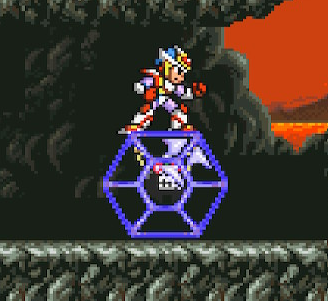
\includegraphics[width=\linewidth]{figures/X2/weapons/C_haunter_2.png}	
	\end{subfigure}
	\caption{Crystal Haunter sub-weapon and trapped enemy.}
\end{figure}

\subsection{
\includegraphics[width=12px, height=10px]{figures/X2/weapons/B_splash.png} Bubble Splash}\label{Bubble_splash}
Bubble Splash is the weapon obtained by defeating Bubble Crab~[\ref{boss:Bubble_crab}]. When used it will fire a stream of bubbles which slightly curve upward as the move and pop if they make contact with enemies.  The number of bubble fired depends on how much the fire button is pressed: a light pressure will cause few bubble to spawn, while an heavier pressure will cause more to spawn, up to seven in total~\cite{wiki:Bubble_splash}. Keeping the fire button pressed will make the weapon fire continuously, making new bubble appear as soon as previous ones pop. When charged this weapon will create several bubble which will orbit around X and damaging enemies which comes in contact to it. However orbitals bubble will keep draining X's energy, only to disappear once it has been all depleted. Furthermore since keeping the fire button pressed is required to charge up the weapon, X will keep shooting bubble in the process, consuming energy while doing so. 

Underwater Bubble Splash will behave slightly differently: fired bubbles will curve upward much faster and, when charged, the weapon will allow X to jump much higher than normal.

\begin{figure}[htp]
	\centering
	\begin{subfigure}{0.4\linewidth}
		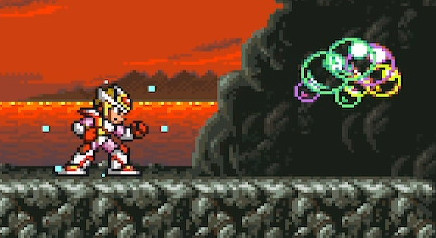
\includegraphics[width=\linewidth]{figures/X2/weapons/B_splash_1.jpg}	
	\end{subfigure}
	\begin{subfigure}{0.275\linewidth}
		
\includegraphics[width=\linewidth]{figures/X2/weapons/B_splash_2.jpg}	
	\end{subfigure}
	\caption{Bubble splash normal fire and charged version.}
\end{figure}

\subsection{
\includegraphics[width=12px, height=10px]{figures/X2/weapons/S_shot.png} Silk Shot}\label{Silk_shot}
By defeating Morph Moth~[\ref{boss:Morph_moth}] X will acquire the Silk Shot. When used X will launch a hunk of garbage in front of him, while when charged X will draw to him a huge mass of scraps, which remains attached to the X buster acting as a shield as long as the fire button remain pressed, only to be release and explode when the button is released.
\begin{figure}[htp]
	\begin{subfigure}{\linewidth}
		\centering
		
\includegraphics[width=0.4\linewidth]{figures/X2/weapons/S_shot_1.png}	
		
\includegraphics[width=0.4\linewidth]{figures/X2/weapons/S_shot_2.png}	
		\caption{Crystals}	
	\end{subfigure}
	\begin{subfigure}{\linewidth}
		\centering
		
\includegraphics[width=0.4\linewidth]{figures/X2/weapons/S_shot_3.png}	
		
\includegraphics[width=0.4\linewidth]{figures/X2/weapons/S_shot_4.png}	
		\caption{Leafs}
	\end{subfigure}
\end{figure}
\begin{figure}
	\ContinuedFloat
	\centering
	\begin{subfigure}{\linewidth}
		\centering
		
\includegraphics[width=0.4\linewidth]{figures/X2/weapons/S_shot_5.png}	
		
\includegraphics[width=0.4\linewidth]{figures/X2/weapons/S_shot_6.png}	
		\caption{Rocks}	
	\end{subfigure}
	\begin{subfigure}{\linewidth}
		\centering
		
\includegraphics[width=0.4\linewidth]{figures/X2/weapons/S_shot_7.png}	
		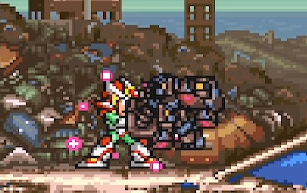
\includegraphics[width=0.4\linewidth]{figures/X2/weapons/S_shot_8.png}	
		\caption{Scraps}
	\end{subfigure}
	\caption{Silk Shot attack types in normal and charged versions.}
\end{figure}


This weapon is probably on of the most gimmicky of the entire series due to its tow features. The first, and most important, one is the fact that damage dealt and projectile type fired by the weapon will change depending on the stage it is used in (charged version remain almost unchanged, save for the type of material drawn), according to following scheme~\cite{wiki:Silk_shot}:
\begin{itemize}
	\item In the \textbf{Energen crystal mine} stage the weapon will shoot a crystal shard which moves in the direction X is facing while bouncing on the floor.
	\item In the \textbf{Weather Control stage} the weapon will fire a pile of leaves  which float upwards. This is the weakest version of Silk Shot.
	\item In the \textbf{Volcanic Zone} and \textbf{Deep Sea base} the weapon will fire a rock projectile, which bounce on the ground a little before exploding.
	\item In all remaining stage the weapon will fire a metal scrap, which explode as soon as it touches a surface, ground included.
\end{itemize}

The second feature of this weapons it its ability to draw health and energy capsule when its charged shot is used inside special rooms in some specific stages.


\subsection{
\includegraphics[width=12px, height=10px]{figures/X2/weapons/S_wheel.png} Spin Wheel}\label{Spinning_wheel}
When using the Spin Wheel, X fires a buzz saw blade which falls on the ground and than crawl along the floor, continuously damaging enemies which comes in contact with it until the blade disappear or the enemy is destroyed. In the latter case the blade will than restart moving forward until it disappears. The saw can also destroy certain blocks and terrains, to open new passages, but only one blade per time can be on screen. When charged, X will release a blade which, instead of moving forward, will split into eight energy bolts traveling in all directions. Bolts pass through obstacles and enemies, dealing damages while also maintaining destructive properties of the uncharged version. This weapon is obtained after defeating Wheel Gator~[\ref{boss:Wheel_gator}].

\begin{figure}[htp]
	\centering
	\begin{subfigure}{0.4\linewidth}
		
\includegraphics[width=\linewidth]{figures/X2/weapons/S_wheel_1.png}	
	\end{subfigure}
	\begin{subfigure}{0.3\linewidth}
		\centering
		
\includegraphics[width=\linewidth]{figures/X2/weapons/S_wheel_2.png}	
	\end{subfigure}
\caption{Spin Wheel normal and charged version.}
\end{figure}

\subsection{
\includegraphics[width=12px, height=10px]{figures/X2/weapons/S_slicer.png} Sonic Slicer}\label{Sonic_slicer}
After defeating Overdrive Ostrich~[\ref{boss:Overdrive_ostrich}] X will gain access to the Sonic Slicer. This weapon fires a spinning blade which travels horizontally at high speed and ricochet on walls with increasing angle of reflection each time, before disappearing once an enemy is hit or it goes offscreen. When charged this weapon fires five blades very close to each other upwards, which than separates and descend down becoming larger in the process.

\begin{figure}[htp]
	\centering
	\begin{subfigure}[t]{0.45\linewidth}
		
\includegraphics[width=\linewidth]{figures/X2/weapons/S_slicer_1.png}	
	\end{subfigure}
	\begin{subfigure}[t]{0.35\linewidth}
		\centering
		
\includegraphics[width=\linewidth]{figures/X2/weapons/S_slicer_2.png}	
	\end{subfigure}
%\end{figure}
%\begin{figure}
%	\ContinuedFloat
%	\centering
	\begin{subfigure}[t]{0.81\linewidth}
		\centering
		
\includegraphics[width=\linewidth]{figures/X2/weapons/S_slicer_3.png}	
	\end{subfigure}
	\caption{Sonic Slicer normal and charged version.}
\end{figure}

\subsection{
\includegraphics[width=12px, height=10px]{figures/X2/weapons/S_chain.png} Strike Chain}\label{Strike_chain}
When using the Strike Chain, X will release a chain with a hook at its end, which can both damage enemies which come in contact with them. How much the chain extends depends on the length the fire button is pressed: a short pressure will cause the chain to extend slightly, while a longer pressure will cause the chain to extend up to its limit. Beside dealing damage, the chain is also able to grub items from distance, enemy drops included, and if a wall is hit, it will pull X towards it. When the weapon is charged X will release a faster and longer chain, which also deals more damage. Furthermore enemies destroyed in this way will always drop an energy pickup for X. This weapon is obtained by defeating Wire Sponge~[\ref{boss:Wire_sponge}]

\begin{figure}[htp]
	\centering
	\begin{subfigure}{0.45\linewidth}
		
\includegraphics[width=\linewidth]{figures/X2/weapons/S_chain_1.png}	
	\end{subfigure}
	\begin{subfigure}{0.45\linewidth}
		\centering
		
\includegraphics[width=\linewidth]{figures/X2/weapons/S_chain_2.png}	
	\end{subfigure}
\end{figure}

\subsection{
\includegraphics[width=12px, height=10px]{figures/X2/weapons/M_mine.png} Magnet Mine}\label{Magnet_mine}
Defeating Magna Centipede~[\ref{boss:Magna_centipede}] allows X to use the Magnet Mine. This weapon fires a single mine which travels at constant speed in the direction it is shot. If the mine makes contact with an enemy it explodes, but if it hits a surface it remains in place for a short time, before exploding. Once a mine attaches to a surface X can immediately fires another one, which can land on the previous one, forming a chain. There is virtually no limit on how many mines X can fires, but typically only four can be shot before the first one explodes. More importantly, the path of each mine can be controlled vertically by inputting up or down, but once a direction is given the mine will follow that direction, meaning that to make it go straight again it is necessary to keep inputting up and down.
\begin{figure}[htp]
	\centering
	\begin{subfigure}[t]{0.4\linewidth}
		
\includegraphics[width=\linewidth]{figures/X2/weapons/M_mine_1.png}	
		\caption{Normal fire}
	\end{subfigure}
	\begin{subfigure}[t]{0.4\linewidth}
		\centering
		
\includegraphics[width=\linewidth]{figures/X2/weapons/M_mine_2.png}	
		\caption{Three mines stacked onto each other.}
	\end{subfigure}
		\end{figure}
	\begin{figure}[htp]
		\ContinuedFloat
		\centering
	\begin{subfigure}[t]{0.4\linewidth}
		\centering
		
\includegraphics[width=\linewidth]{figures/X2/weapons/M_mine_3.png}	
		\caption{Charged version}
	\end{subfigure}
	\begin{subfigure}[t]{0.4\linewidth}
		\centering
		
\includegraphics[width=\linewidth]{figures/X2/weapons/M_mine_4.png}	
		\caption{Absorbing incoming projectiles}
	\end{subfigure}
	\end{figure}
	\begin{figure}[htp]
		\ContinuedFloat
		\centering
	\begin{subfigure}[t]{0.4\linewidth}
		\centering
		
\includegraphics[width=\linewidth]{figures/X2/weapons/M_mine_5.png}	
		\caption{Charged version second stage}
	\end{subfigure}
	\begin{subfigure}[t]{0.35\linewidth}
		\centering
		
\includegraphics[width=\linewidth]{figures/X2/weapons/M_mine_6.png}	
		\caption{Charged version max size}
	\end{subfigure}
	\caption{Magnet Mine sub-weapon.}
\end{figure}
Once charged, the weapon will release a small slow-moving black hole which can be controlled similarly to the base version (see \path{videos/X2/Charged_mine_control.mp4}). The black hole keeps moving forward, passing trough obstacles and enemies (which are still damaged) and absorbing incoming projectile, growing in size in the process up to two stage bigger, but also becoming more difficult to control.



\subsection{
\includegraphics[width=12px, height=10px]{figures/X2/weapons/S_burner.png} Speed Burner}\label{Speed_burner}
Speed Burner releases from the X-buster a pair of intertwined fireballs which travel at high speed in straight direction, disappearing once they collide with an enemy or a surface. In addiction, if Speed Burner is fired while standing on the ground, it will also leave a small trace of fire along its path which deals damage to enemies too. When charged this weapon will wrap X in flames and make him dash forward at high speed, damaging also enemies. When in this state X doesn't take contact damages from enemies, but he does from stage hazards like spikes. This attack can also be used in the air, allowing X to perform an air dash.

Similar to the previous game, this fire weapon behaves differently when used inside water. For the regular attack, in fact, underwater the two fireball won't ignite, and only two small orbs (which deals very small damage) will be shot leaving behind a trail of smoke. For the charged version instead X will simply dash forward, again leaving behind a trail of smoke. When in this state X is not invincible, and will take damage if he makes contact with an enemy.

\begin{figure}[htp]
	\centering
	\begin{subfigure}[t]{0.4\linewidth}
		
\includegraphics[width=\linewidth]{figures/X2/weapons/S_burner_1.png}	
	\end{subfigure}
	\begin{subfigure}[t]{0.4\linewidth}
		\centering
		
\includegraphics[width=\linewidth]{figures/X2/weapons/S_burner_2.png}	
	\end{subfigure}
%\end{figure}
%\begin{figure}
%	\ContinuedFloat
%	\centering
	\begin{subfigure}[t]{0.4\linewidth}
		\centering
		
\includegraphics[width=\linewidth]{figures/X2/weapons/S_burner_3.png}	
	\end{subfigure}
	\begin{subfigure}[t]{0.4\linewidth}
		\centering
		
\includegraphics[width=\linewidth]{figures/X2/weapons/S_burner_4.png}	
	\end{subfigure}
	\caption{Speed Burner sub-weapon attacks outside and inside water.}
\end{figure}

\section{Second Armor}\label{X2:Armor}
Returning from the previous game Dr.~Light's capsules, each one storing a new armor part, which are scattered across four of the eight stages, although this time they are more hidden and often require a specific sub-weapon (or even other parts) in order to get access to them. Furthermore differently from the previous game this game doesn't have any mandatory capsule, making the armor fully optional.
According to \cite{tw:second_armor}\footnote{Translation: \url{https://twitter.com/kobun20/status/1305162448878612480}}, the second armor is actually an improved version of the first one, which X had returned past first game's events. Once returned, Light's capsule analyzed armor's field data in order to upgrade it into an new armor for X.

The second armor is again composed by four main parts, with the addiction of a fifth, secret, one in a similar way the Hadoken was in the first game.

The Second Armor is composed by following components:
\begin{itemize}
	\item Foot parts: When equipped, this parts allow X to perform dashes, already available from the start, in the air too. However air-dashes cannot be performed if X has already dashed on the ground or if he is already dash-jumping. However Foot Parts' air dash flight distance can be extended by combining it with a charged Speed Burner. The capsule containing this power-up is hidden inside the Desert Base, behind a wall breakable only by the Spin Wheel sub-weapon.
	\begin{figure}[htp]
		\centering
			
\includegraphics[width=0.4\linewidth]{figures/X2/Overdrive_ostrich/Ostrich_capsule.jpg}	
			\caption{Foot Parts location}
	\end{figure}	


	\begin{figure}[htp]
		\centering
		
\includegraphics[width=0.4\linewidth]{figures/X2/Morph_moth/Moth_capsule_2.jpg}
		\caption{Body Parts location.}
	\end{figure}
	\item Body Parts: Similarly to the previous game, this power-up increases X's defense by halving all incoming damages to X. Furthermore all damage dealt to X will also increase a special gauge which, one full, allows X to perform the \textit{Giga Crush} attack, which heavily damages all enemies on screen. 
	However the gauge doesn't refill between stages, meaning the only way to store energy is by getting hit. The capsule containing Body Parts is hidden in the Robot Junkyard stage, under a floor at the beginning of the stage breakable only with the Spin Wheel sub-weapon.
	\begin{figure}
		\centering
		
\includegraphics[width=0.4\linewidth]{figures/X2/weapons/G_crush_1.png}
		\caption{Giga Crush attack}
	\end{figure}.
	
	\begin{figure}[htp]
		\centering
		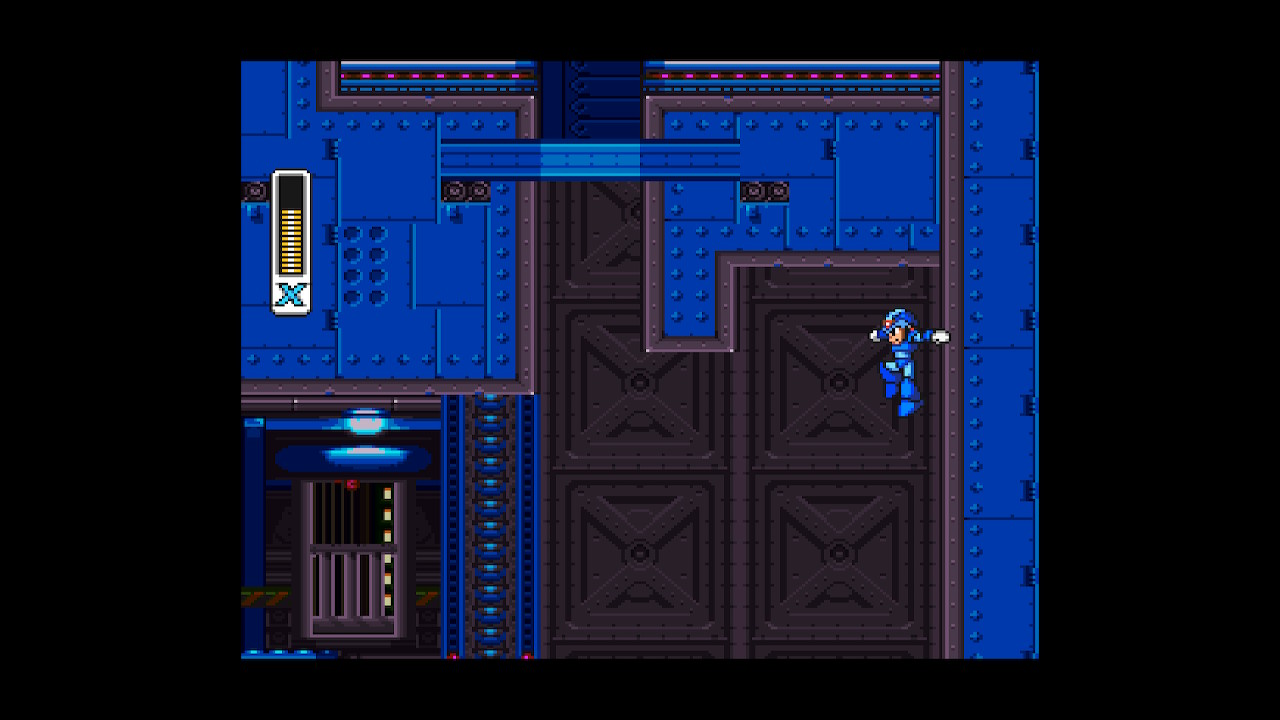
\includegraphics[width=0.4\linewidth]{figures/X2/Wheel_gator/Gator_capsule.jpg}\\
		\caption{Arm Parts location .}
	\end{figure}
	\item Arm Parts: This upgrade allows X to use two X-buster when using charged shot. When charging, X will be able to pass the second charge level, accumulating energy in the second Buster, up to other two level.  When the player release the fire button, X will shoot a first charged shot (depending on the charge level reached) and will remain flashing until the fire button is pressed again, making X release a second, fully charged, shot. Most importantly, if the player release the two charged shot in rapid succession, they can combo against all enemies, bosses included, ignoring their invincibility frame and dealing massive damage. This upgrade is stored inside Wheel Gator stage, inside a chamber accessible only via wall jumping from an opening on the roof, and can be obtained either via precise wall-jumping, by using the the Giga Crush to extend X's airborne period, by using the Strike Chain to pull X towards the wall (\path{videos/X2/Buster_capsule_chain.mp4}), or simply by using the air dash to reach the opening.
	\begin{figure}
		\centering
		
\includegraphics[width=0.6\linewidth]{figures/X2/weapons/Double_shot.png}
		\caption{Double charged shot.}
	\end{figure}

	\item Head Parts: The Head Parts allow X to use the item tracer, a radar which X can fire and will point in direction of the closest secret in the level. Secrets pointed include hidden passages and items (such as ), heart tanks and sub-tanks, other Light's capsules and refill rooms. Despite showing an ammunition gauge, this upgrade does not use any energy. The capsule with the Head Parts is hidden in Crystal Snail's stage, at the end of a secret path found while sliding down a pit after the stage's sub-boss.
	\begin{figure}[htp]
		\centering
		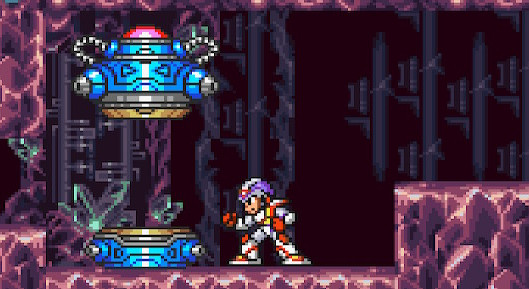
\includegraphics[width=0.4\linewidth]{figures/X2/Crystal_snail/Crystal_capsule.jpg}
		
\includegraphics[width=0.345\linewidth]{figures/X2/weapons/Tracer.png}
		\caption{Head Parts location and Item Tracer.}
	\end{figure}

	\begin{figure}[htp]
		\centering
		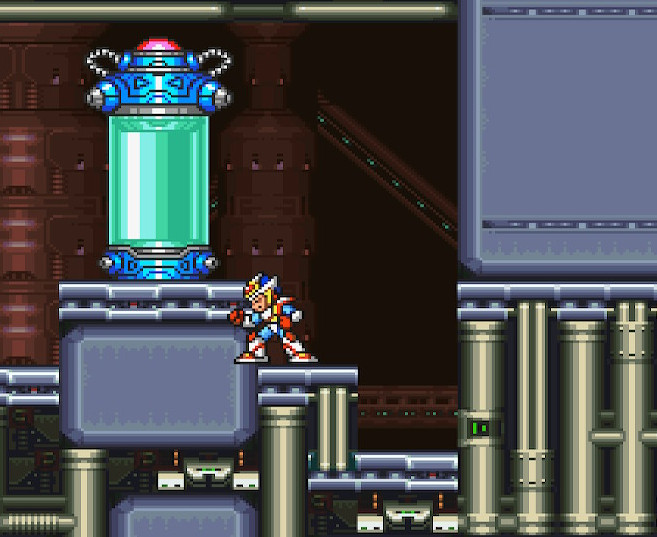
\includegraphics[width=0.4\linewidth]{figures/X2/Haunter_stages/Shuryuken_capsule.jpg}
		
\includegraphics[width=0.335\linewidth]{figures/X2/weapons/Shoryuken.png}
		\caption{Shoryuken's capsule location and attack.}
	\end{figure}
	\item Shoryuken\label{shoryuken}: Similarly to X1's Hadoken, this secret upgrade is the prize for collection all other power-up items (Zero's parts do NOT count). Once obtained, X will be able to perform the fire uppercut from the \textit{Street Fighter} series by inputting the command $\rightarrow$, $ \downarrow$, $\searrow$ (with X facing left) + fire button but ONLY if X is at full health and on the ground. Differently from the previous technique, however, is the fact that the damage dealt by this technique is dependent on the number of frame the attack makes contact with an enemy, meaning that a misplaced Shoryuken can fail to insta-kill bosses. To be precise, Shoryuken deals 16 damage to enemies without invincibility frame and 8 otherwise and the damage is applied every two frames, meaning that in order to kill a boss at full health (32 hit points) 5 frame of contact are needed (16 damage the first frame, than zero the second, 8 the third, than again 0 on fourth and last 8 at the fifth). 
	 This upgrade can be found inside the third X-haunter stages, at the end of a secret passage full of spikes which requires precise air dash. In order to obtain this capsule, moreover, X has to reach it with full health (but there are no limitation on Sub-tank status).
\end{itemize}

\section{Opening Stage}
Being the first stage in the game, this level act as a tutorial for the player to (re-)learn basic game mechanics. The stage begins with a short scene where X and other Haunters are riding their vehicles to the factory, but are attacked by a fierce resistance. X than jumps off his bike, which crashes onto and enemy, and proceeds on feet. From here the player gains X's control and can start moving. Attention must be done immediately, however, since the enemy on which the bike crashed on is still alive and will shoot X immediately. Past this first obstacle the player will enter the factory where other enemies lies ahead, such as \hyperlink{enem:Bar_Waying}{Bar Waying} which do not deal damages but use their body to block the path and require several shot to be destroyed. Traversing the factory X will find himself onto a production line, which uses conveyor belts to move manufactured mavericks from one construction bay to the other (three in total); if X get caught inside one of they bays he will receive damage, while if he pass over it the bay will simply upgrade the constructed maverick which, in case of the third and last bay, will activate and attack X. Passes this section a last one awaits which consists in a wall-jump tutorial: at the bottom of the room where X starts a \hyperlink{enem:Slidame}{Slidame} is also present. This enemy as soon as it detects X will rush at the top of the room and begin closing the walls in an attempt to crush X. Although not very fast, the player as to climb the wall quickly in  order to no get killed by the wall. Should instead the player fall down back to the room's bottom and the wall close it will be sufficient to return back in the stage a little, in order to reset the room as it was before, giving another chance to climb. Once reached the top of the room a small corridor awaits, ending in a deep pit which X has to jump into, as at the end a boss door awaits.

Beside enemies already cited, this level also house following enemies~\cite{wiki:X2_opening}:
\begin{itemize}
	\item \hyperlink{enem:Bar_Waying}{Bar Waying}
	\item \hyperlink{enem:Cannon_Driver}{Cannon Driver}
	\item \hyperlink{enem:Mecha-Arm}{Mecha-Arm}
	\item \hyperlink{enem:Scrambler}{Scrambler}
	\item \hyperlink{enem:Scriver}{Scriver}
	\item \hyperlink{enem:Slidame}{Slidame}
\end{itemize}

\subsection{Giant Mechaniloid CF-0}
Differently from the previous game, this opening stage ends in a boss fight the player has to win. The boss in question is the giant mechaniloid CF-0, an enormous robot created by the X-Haunters with the purpose of mass production and conquer cities around the world, although due its weight the movement speed is reduced to the minimum. X-Haunters' plans where however halted by Maverick Haunters's attack, which forced them to activate the only completed mechaniloid to try stop the attack, but resulting only in its destruction by the hands of X.

Despite its size, the fight against CF-0 is relatively simple. The boss room is very big and and filled with platform at various level, connected by ladders to allow X to climb up should he fall down, and this allow X to easily dodge the two attacks this boss can perform: a spiked fist which aims at player's current position and a jump attack where CF-0 aims to land onto X. However both of these attacks can be easily avoided by keep moving between top platforms and deals minimal damage o X. It is in fact on the upper side of the room that X should stay to damage the boss, as its only weak point is the head, which happens also to be one of the three body parts that can damage X if he makes contact with them, the other ones being CF-0's arms and feet. All the rest of its body does not deal any damage of sort, acting like background. Finally, and having the healthbar of a boss, CF-0 takes massive damage from X's charged shot, which can destroy it in four shots.


\begin{figure}[htp]
	\centering
	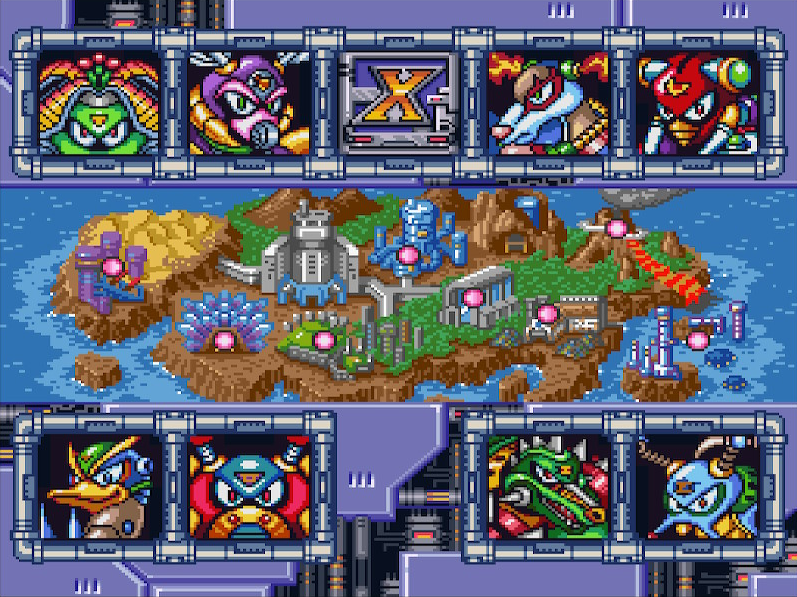
\includegraphics[width=0.5\linewidth]{figures/X2/map.png}
	\caption{Full map with Bosses and their locations}
\end{figure}


\section{Weather Control}
The first stage the game present is the weather control stage. As the name suggest, focus of the stage are weather conditions, which can change an be controlled as the stage progress in order to affect X's mobility or enemies' behavior. The source of said weather changes is to be found in an element presented right at the beginning of the level: \hyperlink{enem:Weather_crystal}{weather crystals}. Although these items are considered enemies, they won't hurt X in any way, even if he makes contact with them. What they will do, instead, is changing the weather in the portion of the level X is in, affecting X's movement and changing enemies' behavior and power. While this can only appear to be a cons, the truth is X can manipulate said enemies to obtain a favorable weather to ease the stage exploration. There are a total of four crystals in the stage, each one with a default weather set which can be changed depending on the weapon X uses to hit it, according to following list~\cite{wiki:Weather_crystal}:
\begin{itemize}
	\item \textbf{Cloudy weather}: Obtained hitting the crystal with the Strike Chain weapon (the crystal turns yellow). In this state all enemies are active and \hyperlink{enem:Sky_farmer}{sky farmers} plant \hyperlink{enem:Sabottein}{sabotteins}, which only grow half-size.
	\item \textbf{Warm/Sunny weather}: Obtained by hitting the crystal with the Speed Burner (the crystal turns orange). In this state all enemies are active, but \hyperlink{enem:Croak_hopper}{croak hoppers} will overheat and explode, while planted \hyperlink{enem:Sabottein}{sabotteins} will growth to their full size.
	\item \textbf{Rainy weather}: Obtained by hitting the crystal with the Bubble Splash (the crystal turns cyan). In this state \hyperlink{enem:Croak_hopper}{croak hoppers} will actively move for the stage instead of staying in place, while planted \hyperlink{enem:Sky_farmer}{sky farmers} will release \hyperlink{enem:Rightod}{rightods} to chase X. \hyperlink{enem:Sole_solar}{sole solars} will instead remain deactivated. Finally in rainy weather a constant, inverse, speed is applied to X while moving, resulting in a slower walking and running speed, as well as a shorter jump distance.
	\item \textbf{Foggy weather}: Obtained by using the Crystal Haunter on the crystal (it turns purple/black). In this state all enemies are deactivated.
\end{itemize}

\begin{figure}[htp]
	\centering
	\begin{subfigure}{0.3\linewidth}
		\centering
		
\includegraphics[width=\linewidth]{figures/X2/Wire_sponge/sponge_crystal_default.jpg}
		\caption{Intact crystal}
	\end{subfigure}
	\begin{subfigure}{0.3\linewidth}
		\centering
		
\includegraphics[width=\linewidth]{figures/X2/Wire_sponge/sponge_crystal_cloud.jpg}		
		\caption{Cloudy}
	\end{subfigure}
	\begin{subfigure}{0.3\linewidth}
		\centering
		
\includegraphics[width=\linewidth]{figures/X2/Wire_sponge/sponge_crystal_sun.jpg}
		\caption{Sunny}
			\end{subfigure}
	\begin{subfigure}{0.3\linewidth}	
		\centering
		\includegraphics[width=\linewidth]{figures/X2/Wire_sponge/sponge_crystal_rain.jpg}\\
		\caption{Rainy}
	\end{subfigure}
	\begin{subfigure}{0.3\linewidth}
		\centering
		\includegraphics[width=\linewidth]{figures/X2/Wire_sponge/sponge_crystal_fog.jpg}
		\caption{Foggy}	
	\end{subfigure}
	\begin{subfigure}{0.3\linewidth}
		\centering
		\includegraphics[width=\linewidth]{figures/X2/Wire_sponge/sponge_crystal_broken.jpg}
		\caption{Broken crystal}	
	\end{subfigure}
	\caption{Different states of weather condition and crystals.}
\end{figure}
Should the player destroy a crystal weather conditions for the stage's portion will be set at random.

The first crystal the player finds is near the beginning of the level, in a very straightforward section with only some enemies to stop X and that ends with a second weather crystal, opening to the second part of the level. Here floating platform will move up and down over a spiky pits, and X has to move from one to another paying attention as platforms are taller than wider, meaning the best way to stay on them is by wall-jumping. The main difficulty in this section is given by the default weather set, which is the rain that will reduce X's jump distance, making harder to pass from one platform to the next one. After this section an elevator awaits to bring X upper in the stage where a third section awaits. This part is very similar to the first one, only with more enemies and spiky pits the last two weather crystals, which will activate different enemies as the player proceed. Once this part has been passed, a climbing section awaits, with platforms with enemies on top and connected by ladders ending in a corridor which brings to the boss door.

Following enemies occupy the stage~\cite{wiki:weather_control}
\begin{itemize}
	\item \hyperlink{enem:Aclanda}{Aclanda}
	\item \hyperlink{enem:Croak_hopper}{Croak Hopper}
	\item \hyperlink{enem:Rightod}{Rightod}
	\item \hyperlink{enem:Sabottein}{Sabottein}
	\item \hyperlink{enem:Scriver}{Scriver}
	\item \hyperlink{enem:Sky_farmer}{Sky Farmer}
	\item \hyperlink{enem:Sole_solar}{Sole Solar}
	\item \hyperlink{enem:Weather_crystal}{Weather Crystal}
\end{itemize}

\subsection{Heart Tank}
The Heart Tank is hidden immediately at the beginning of the stage. By climbing the leftmost wall of the beginning room, the player will find a small entrance in the top corner with the Heart Tank inside it.
\begin{figure}[htp]
	\centering
	\includegraphics[width=0.5\linewidth]{figures/X2/Wire_sponge/Sponge_heart.jpg}
	\caption{Heart Tank location.}
\end{figure}

\subsection{X-Haunters' room}
When reaching the elevator section, if the player manages to make X sneak under the elevator a new path will open, leading to the X-Haunters room
\begin{figure}[htp]
	\centering
	\includegraphics[width=0.5\linewidth]{figures/X2/Wire_sponge/Sponge_haunter_room.jpg}
	\caption{X-Haunters room location.}
\end{figure}

\subsection{Sub Tank}
In the rain section, if instead of proceeding by platforming the player uses the first one to jump onto the wall on the right (where the second crystal is found) and climb it, it will reach a new path over the default one made of logs separated into two main platforms. At the end of the second one is where the Sub Tank resides.  
\begin{figure}[htp]
	\centering
	\includegraphics[width=0.5\linewidth]{figures/X2/Wire_sponge/Sponge_tank.jpg}
	\caption{Sub Tank location.}
\end{figure}

\subsection{Wire Sponge}\label{boss:Wire_sponge}
Wire Sponge (the ``Little Forest Demon''~\cite{book:MMX_Complete_art}) was a sponge cucumber-based Maverick manufactured inside one of Sigma's factories although born from an accident. Because of a design mistake, in fact, Wire Sponge was build with a personality disorder which made him childish, cheerful and easily amused, with the love for dancing and playing. Although this personality was not tailed for army, Wire Sponge's strength  and violence was uncontested, and X-Haunters put that in use by making him conquer the weather control center which he uses as his own playground, changing the weather as he please~\cite{wiki:wire_sponge},\cite{wayback:X2_resources}.

In battle, Wire Sponge mainly attacks by swinging his chord, the Strinke Chain in various way to damage X.
When Wire Sponge spin his chain he will deflect all incoming projectiles, so attacking while in this state is useless. After spinning the chain, Wire Sponge will almost always attack by throwing it at X and, if the chain hits a wall, he will be pulled towards it. Other times Wire sponge will instead throw the chain on the ceiling and start climbing it, while firing seeds from his head aiming at X. When a seed its a wall or the floor (not the roof, of which the seed will ricochet on) it will grow into a spiked vine which damages X on contact. These spikes can be destroyed by any weapon and doing it is a suggested action, since after four vine are planted Wire Sponge will drop down~\cite{rta:x2} terminating his attack which leaves him very open for damages, so the longer he performs it the better. Finally once Wire Sponge's health drops below 10 points he will start using his desperation moves. With this moves his flower becomes a lightning rod from which he will make lightning fall in the room but they can be easily avoided as they fall at the same distance every time and never near the boss himself, so staying close is a good strategy to avoid taking damage. However once this attack is performed Wire Sponge will become charged with electricity which will increase his damage output.

\begin{figure}[htp]
	\centering
	\begin{subfigure}{0.4\linewidth}
		\centering
		\includegraphics[width=\linewidth]{figures/X2/Wire_sponge/Sponge_spin.png}
		\caption{Spinning the chain}
	\end{subfigure}
	\begin{subfigure}{0.5\linewidth}
		\centering
		\includegraphics[width=\linewidth]{figures/X2/Wire_sponge/Sponge_pull.jpg}
		\caption{Being pulled to the wall}
	\end{subfigure}
	\begin{subfigure}{0.4\linewidth}
		\centering
		\includegraphics[width=\linewidth]{figures/X2/Wire_sponge/Sponge_hang.jpg}
		\caption{Hanging and launching seeds (bottom left: a sprouted vine)}
	\end{subfigure}
\end{figure}
\begin{figure}
	\ContinuedFloat
	\centering
	\begin{subfigure}{\linewidth}
		\centering
		\includegraphics[width=0.4\linewidth]{figures/X2/Wire_sponge/Sponge_phase2.jpg}
		\includegraphics[width=0.4\linewidth]{figures/X2/Wire_sponge/Sponge_DM.jpg}
		\caption{Charging and releasing his desperation move}
	\end{subfigure}
	\begin{subfigure}{0.4\linewidth}
	\centering
	\includegraphics[width=\linewidth]{figures/X2/Wire_sponge/Sponge_charged.jpg}
	\caption{Powered up by electricity}
	\end{subfigure}
	\begin{subfigure}{0.28\linewidth}
	\centering
	\includegraphics[width=\linewidth]{figures/X2/Wire_sponge/sponge_cut.jpg}
	\caption{Cut in half.}
	\end{subfigure}

	\caption{Wire Sponge's attacks.}
\end{figure}

Wire Sponge is often considered an easy boss due the long time he makes himself vulnerable when he hangs from the ceiling and the fact that all his others attacks are easy to dodge. This makes fight him with only the buster relatively safe, also since his main weakness, the Sonic Slicer doesn't do much more to him than increased damage (and a different animation when it is used to defeat him).

According to in-game data, Wire Sponge possess a power of 6400 rp and a speed of 4800 rp, and upon defeating him X will gain access to the Strike Chain~[\ref{Strike_chain}].
\begin{table}[htp]
	\centering
	\begin{tabular}[h]{l c c}
		
		\toprule
		\multicolumn{2}{c}{Health}  & 32\\
		\midrule
		\multicolumn{1}{c}{Attack} & \multicolumn{1}{c}{Damage}& \multicolumn{1}{c}{Damage-electrified}\\
		Contact & 5 & 7\\
		Strike Chain & 2 & 4\\
		Seed/Vines& 2&-\\
		Lightnings & 2&-\\
		\bottomrule
	\end{tabular}
	\caption{Wire Sponge's attack's damages~\cite{wiki:wire_sponge}}
\end{table}

\section{Robot Junkyard}
As the name suggest, the Robot Junkyard stage takes place inside a scrapyard where old robot are demolished.

The beginning of the stage corresponds to the junkyard's entrance. From here it is already possible to see how most of enemies in the level will present themself: most of them will be, in fact, old robot ready to be destroyed or repaired in some way which will attack X as he come closer.  Passed the entrance  there is a long corridor full with enemies and a magnet on the roof which pulls metal upwards thus enhancing X's jump capabilities, but this little bonus is totally useless, as there are no pits in this section. Passed the corridor there is a small climbing section where six big platforms are placed on the opposite side of a large gap, and X has to dash-jump from one to another in order to avoid falling and returning to the beginning of the room.

Once this rooms has also been passed the player will face the first sub-boss of the stage: entering inside the capsule room will in fact trigger the door closure and free from the capsule itself a \hyperlink{miniboss:Paraloid_S-38}{Paraloid S-38} which will possess and \hyperlink{miniboss:Old_robot}{Old Robot}. This enemy is heavy armored and X's attack will bounce off it unless aimed at its center, the only spot which can take damage. Old Robot's main attacks consist in moving toward X by performing small jumps, make a big jump in the air and dive onto X and occasionally firing junk projectiles. Although the sub-boss itself may not appear as dangerous as other ones, the real difficulty of the battle comes from its possible-endless duration. As the Old Robot is destroyed (easily done by using a charged Spin Wheel, if available) the Prarloid S-38 will exit the robot's body and immediately dive into the ground in order to resurrect another one, basically resetting all player's progress in the boss fight. In order to avoid this a well-aimed Charges Shot or, even better, Speed Burner are sufficient to defeat the small insect and open the exit door.

Once outside the sub-boss rooms a long ladder will bring X deeper in the stage, to a small platforming section where enemies on top of platform will try to mess with X's jumps to make him fall into one of the few spiked pits of the stage. Passed the portion of the level another corridor, similar to the first one met, awaits. However here magnets will work in the opposite way respect the first one, reducing X's jump height, but again this can be totally ignored, as no platforming is required in the section. At the end of the corridor a ladder awaits to bring X a level lower in the stage inside a room where a second combination of  \hyperlink{miniboss:Paraloid_S-38}{Paraloid S-38} and \hyperlink{miniboss:Old_robot}{Old Robot} has to be fought again as second sub-boss of the stage to access, upon its defeat, to the last stage's corridor before the boss room.

Following enemies appears in the stage~\cite{wiki:Robot_Junkyard}:
\begin{itemize}

	\item \hyperlink {enem:Cannon_Driver}{Cannon Driver}
	\item \hyperlink {enem:Disk_Boy_08}{Disk Boy 08}
	\item \hyperlink {enem:Garakuta_Robot}{Garakuta Robot} 
	\item \hyperlink {enem:Hanged_Reploid}{Hanged Reploid}
	\item \hyperlink {enem:Pararoid_R-5}{Pararoid R-5}
	\item \hyperlink {miniboss:Paraloid_S-38}{Paraloid S-38} and \hyperlink{miniboss:Old_robot}{Old Robot}
	\item \hyperlink {enem:Pararoid_V-1}{Pararoid V-1}
\end{itemize}


\subsection{Heart Tank}
Near the beginning of the stage, before entering the junkyard facility the player will spot a \hyperlink {enem:Disk_Boy_08}{Disk Boy 08} on top of a platform. By trapping it with the Crystal Haunter it is possible to create a higher platform for X to jump on and, from the top of it, dash jumping onto the upper part of the junkyard entrance where a life up and the heart tank are hidden. Alternatively if the player is capable of performing a \emph{Neon Jump} (see sec. \ref{Neon_jump} for more details) it can use it to reach the upper level without having to obtain the Crystal Haunter weapon first.

\begin{figure}[htp]
	\centering
	\begin{subfigure}{0.305\linewidth}
	\centering
	\includegraphics[width=\linewidth]{figures/X2/Morph_moth/Moth_heart_1.jpg}	
	\caption{}
	\end{subfigure}
	\begin{subfigure}{0.4\linewidth}
		\centering
		\includegraphics[width=\linewidth]{figures/X2/Morph_moth/Moth_heart_2.jpg}
		\caption{}	
	\end{subfigure}
	\caption{Heart Tank location: from (a) it is necessary to reach the upper-right wall in order to reach (b). Using a crystal haunter on the enemy which stands on where X is is the intended way.}
\end{figure}


\subsection{Light's Capsule}\label{X2:Body_parts}
In the first magnetized roof section, near its end if the player uses the Item Tracer power-up from the helmet the radar will point at a specific position on the floor. If the player releases in that spot a Spin Wheel (normal or charged), the blade will start digging in the terrain, opening a new path which leads to the armor capsule holding the body upgrade. The item tracer is not mandatory, as experienced player can open the passage directly.
\begin{figure}[htp]
	\centering
	\begin{subfigure}{0.4\linewidth}
		\centering
		\includegraphics[width=\linewidth]{figures/X2/Morph_moth/Moth_capsule_1.jpg}	
		\caption{}
	\end{subfigure}
	\begin{subfigure}{0.4\linewidth}
		\centering
		\includegraphics[width=\linewidth]{figures/X2/Morph_moth/Moth_capsule_2.jpg}
		\caption{}	
	\end{subfigure}
	\caption{Armor Capsule's location. From (a) the Spin Wheel will open a passage up to (b).}
\end{figure}



\subsection{X-Haunters' room}
In the long ladder section if instead of dropping down directly X jumps to the right he will find a corridor leading to the Huanter's room.

\begin{figure}[htp]
	\centering
	\includegraphics[width=0.8\linewidth]{figures/X2/Morph_moth/Moth_haunter_room.jpg}
	\caption{X-Haunters's room location}
\end{figure}

\subsection{Morph Moth}\label{boss:Morph_moth}
Morph Moth was a mysterious reploids with an unknown past and affiliation. An experimental prototype, Morph Moth was built with the special capability  of powering himself up by absorbing scraps, in order to evolve from his cocoon form to the adulthood~\cite{wiki:Morph_moth},\cite{wayback:X2_resources}. This particular features caught Sigma' interests, which enrolled him into his army on to be deployed by the X's haunter during their revolution. The plan was to use Moth's special ability in controlling scraps to resurrect and create new mavericks for their army. However Morph Moth never showed any particular interest in his work.

The battle against Morph Moth is split into two phases, the cocoon form being the first. While in this state Moth will perform three attack cyclically. The first attack is the Scrap Scatter, where Morph Moth swings at increasing speed scattering scraps around, only to fall down when the speed is high enough to break the string. At this point Moth will being to attack with his Dash Scrap Scatter, moving underground from one side to the arena to the other while scattering more scraps as he goes. Finally he will re-hang himself to the ceiling and start performing his Scrap Absorption attack, absorbing scrap in clockwise or counter-clockwise way at high speed, increasing in size in the meanwhile. 

\begin{figure}[htp]
	\centering
	\begin{subfigure}{0.3\linewidth}
		\centering
		\includegraphics[width=\linewidth]{figures/X2/Morph_moth/Moth_1.jpg}
	\end{subfigure}
	\begin{subfigure}{0.3\linewidth}
		\centering
		\includegraphics[width=\linewidth]{figures/X2/Morph_moth/Moth_2.jpg}
	\end{subfigure}
	\begin{subfigure}{0.3\linewidth}
		\centering
		\includegraphics[width=\linewidth]{figures/X2/Morph_moth/Moth_3.jpg}
	\end{subfigure}
	\vspace{2pt}
	\begin{subfigure}{0.3\linewidth}	
		\centering
		\includegraphics[width=\linewidth]{figures/X2/Morph_moth/Moth_4.jpg}
	\end{subfigure}
	\begin{subfigure}{0.3\linewidth}
		\centering
		\includegraphics[width=\linewidth]{figures/X2/Morph_moth/Moth_5.jpg}	
	\end{subfigure}
	\begin{subfigure}{0.3\linewidth}
		\centering
		\includegraphics[width=\linewidth]{figures/X2/Morph_moth/Moth_6.jpg}
	\end{subfigure}
	\caption{Different stages of Morph Moth's growth.}
\end{figure}

The second phase of the boss fight can be triggered in two ways. The first (and often seen) one is by bringing Moth's health below 75\%, while the second one can be achieved by leaving him absorb enough scraps to achieve full-size (if left performing his attacks, the player will note that Moth's cocoon will increase in size). One one of these conditions are met, Morph Moth will exit the arena destroying the ceiling, to reappear shortly after in his Moth form. In this second phase Morph Moth has only two attacks he'll perform while flying around: the first one is the Phosphorescent Powder, where he will start gliding down leaving behind a trace of scales which slowly descends and damage X on contact; the second one is the Beam attack, where he fires a powerful beam aiming at player's position~\cite{book:Compendium}.


\begin{figure}[htp]
	\centering
	\begin{subfigure}{0.4\linewidth}
		\centering
		\includegraphics[height=3.5cm]{figures/X2/Morph_moth/Moth_swing.jpg}
		\caption{Swinging}
	\end{subfigure}
	\begin{subfigure}{0.5\linewidth}
		\centering
		\includegraphics[height=3.5cm]{figures/X2/Morph_moth/Moth_underground.jpg}
		\caption{Dashing underground}
	\end{subfigure}
	\begin{subfigure}{0.4\linewidth}
		\centering
		\includegraphics[width=\linewidth]{figures/X2/Morph_moth/Moth_powder.jpg}
		\caption{Phosphorescent Powder}
	\end{subfigure}
\end{figure}
\begin{figure}
	\ContinuedFloat
	\centering
	\begin{subfigure}{0.4\linewidth}
		\centering
		\includegraphics[height=5cm]{figures/X2/Morph_moth/Moth_beam.jpg}
		\caption{Beam}
	\end{subfigure}
	\begin{subfigure}{\linewidth}
		\centering
		\includegraphics[height=4cm]{figures/X2/Morph_moth/Moth_burn.jpg}
		\includegraphics[height=4cm]{figures/X2/Morph_moth/Moth_hurt.jpg}
		\caption{Burnt in cocoon form and hurt in Moth form}.
	\end{subfigure}
	\caption{Morph Moth's attacks.}
\end{figure}


Battling Morph Moth without taking much damage can be hard. In his cocoon form the scraps he tosses around will be thrown randomly, so quick reflexes are needed to avoid them, while to dodge the absorption attack quick and precise wall jumps have to be made in order to jump from one side of the arena to the other, while also avoiding to land on the boss. In the second phase, instead, Moth will continuously perform attacks, alternating between the two he has, which can be difficult to dodge: the scales cover a wide area, while the beam comes out fast and aims at the player, which could find difficult to dodge if already dealing in avoiding the scales. Furthermore in this phase Moth's attacks is increased, meaning  he can deal many damages in a short amount of time. Moth's weakness is the Speed Burner, which will set him on fire dealing heavy damages and stunning him, but it does not have any other effects, meaning the boss will keep performing all his attacks in order without any limitation.

Also labeled the ``\textit{Fallen Angel from the Island of Dreams}''~\cite{book:MMX_Complete_art}, Morph Moth possess a power equal to 3200 rp and a speed of 8800 rp. Once defeated X will gain access to the Silk Shot (\ref{Silk_shot}) which, ironically, is able to destroy most enemies found in the stage in one hit, sub-bosses included.


\begin{table}[htp]
	\centering
	\begin{tabular}[h]{l c}
		
		\toprule
		\multicolumn{1}{c}{Health}  & 32 \\
		\midrule
		\multicolumn{1}{c}{Attack} & \multicolumn{1}{c}{Damage}\\
		Contact - Cocoon & 4 \\
		Contact - Moth& 8\\
		Scraps (any) & 2\\
		Phosphorescent Powder& 2\\
		Beam & 2\\
		\bottomrule
	\end{tabular}
	\caption{Morph Moth's attack's damages~\cite{wiki:Morph_moth}}
\end{table}

\section{Volcanic Zone}
The Volcanic Zone Stage is, among all other stages, the one which will test the most the player's ability in climbing and wall jumping~\cite{stratwiki:Volcanic_zone}. 

The stage's beginning is relatively easy, as no enemies are present except for a single \hyperlink{enem:Beetron}{Beetron}, which will move up and down until X reaches its same vertical height. At that point it will ram into X and, if it hits a breakable wall Beetron will destroy it opening a passage but also destroying itself in the process. Beside opening new passages X can also stand onto Beetron, as they have a platform on top.

Whether X enters the volcano from the top or by breaking the bottom-left wall (in this case the player will found a small passage with healing items) the next stage's section take place inside the active volcano. After some enemies on the walls X will reach a metallic floor and the screen will start shaking. From that moment the lave will begin rising, leaving as only way to escape climbing to the volcano's top. To do this the player must be very quick and precise in wall jumping, as the exit conduit is not regular but presents several narrowing and ledges which requires to continuously pass from a wall to the other. Once reached the top the lava will continue to erupt upwards, allowing X to keep going without worrying of the lava anymore.

The third section is another outside one, where the player has to platform between rock pillars, which will begin collapsing into the lava as soon as X touches them. At the section's end a second Beetron can be found, which can be used to open one of the two blocked passages (one above and one below the main one) for the second indoor section. Here the first part requires again some platforming between collapsing pillars onto a lava pool in order to reach the last climbing section and exit the volcano. In this climb part there is no lava chasing X, so there is no hurry to exit, but the section is full of pipes which constantly emits gas that can be set on fire when a \hyperlink{enem:Morgun}{Morgun} enemy lands near a pipe. The fire lasts for some time and deals heavy damage to X, so disposing of these enemies is suggested. The gas itself does not damages X, so standing in front of it is safe.

Once exited from the second volcano, by going a little further to the right the player will find the boss door.

Following enemies appears in the level~\cite{wiki:Volcanic_zone}
\begin{itemize}
	\item \hyperlink{enem:Bar_Waying}{Bar Waying}
	\item \hyperlink{enem:Barite_Lastar}{Barite Lastar}
	\item \hyperlink{enem:Beetron}{Beetron}
	\item \hyperlink{enem:Morgun}{Morgun}
\end{itemize}


\subsection{Sub Tank}
Right at the beginning of the stage if the player manages to reach the entrance to the volcano without destroying the Beetron, and from there jump on to the platform this enemies carry on, the Beetron will move backwards until it reaches a hidden zone on the top left of the map, where the Sub Tank resides. 
\begin{figure}[htp]
	\centering
	\includegraphics[height=5cm]{figures/X2/Flame_stag/Stag_tank.png}
	\caption{Sub Tank location.}
\end{figure}


\subsection{Heart Tank}
While escaping from the lava in the first volcano the player will immediately notice the Heart Tank, in plain sight on one of the many narrowing while climbing. Reaching this collectible can be difficult, not only due the lava chasing the player, which will kill X if he is too slow, but also for the Bar Waying enemy which will act as a wall, slowing down the process to get it even further. The best way to get this item is to climb as fast as possible and dispose of the Bar Waying as soon as he appears by using weapons such as Spin Wheel, Magnet Mine or Silk Shot.
\begin{figure}[htp]
	\centering
	\includegraphics[height=5cm]{figures/X2/Flame_stag/Stag_heart.png}
	\caption{Heart Tank location.}
\end{figure}

\subsection{X-Haunters' room}
When entering in the second volcano, if the player uses the second Beetron to destroy the upmost wall two possible passages will open: by going down the player will return to the main route and continue in the level, while going up the player will find the X-Haunter's room.
\begin{figure}[htp]
	\centering
	\includegraphics[height=5cm]{figures/X2/Flame_stag/Stag_haunter_room.png}
	\caption{X-Haunters' room location location.}
\end{figure}


\subsection{Flame Stag}\label{boss:Flame_stag}

Flame Stag once belonged to the 17$^{th}$ Elite Unit, where he fought alongside his friend Boomer Kuwanger.  When the rebellion began the two friends defected together, but Flame Stag became missing shortly after, whereas his friend ended up as shown in sec.~\ref{boss:Boomer_Kuwanger}. Six Month later his mysterious disappear, Flame Stag reappeared, aiming to make erupt the Volcanic zone, obscuring the sun with the ashes and give start to a new ice age. If his plan is somehow connected with X-Haunter activities is unknown.

Also known as the ``\textit{Heat Knuckle Champion}''~\cite{book:MMX_Complete_art}, Flame Stags stays faithful to his nickname and the animal he is based on by fighting with fast fire-based melee attacks in rapid succession. He will often begin the fight by performing his triangular kick attack to rapidly climb the arena's wall (which for this battle is much taller, similar to Morph Moth's one) and chasing X if he tries to climb them to avoid him. Should X instead stay on the ground Stag will perform only few jumps and then come down, where he will perform one of his remaining two attacks, these being the Speed Burner in projectile mode, where he shoots two fireball projectiles the first one which slightly descends and the second one which rises and can also climb walls, and the Speed Burner in Body Blow mode, where Flame Stag dash towards the player covered in fire and, if it hits, it will launch X in the air with a powerful uppercut. This attack also leaves behind a trail of fire which also deals damage. Finally, as most bosses of the game, if Flame Stag drops below under 50\% of health he will activate his last resort, in this case being the Super Mode. While in this state (which last for the remaining of the fight) Flame Stag's flame turn blue, corresponding to an increase of movement and attack speed as well as the addition of another attack following the uppercut, which consist slamming X onto the ground after sending him fly with the first attack.

\begin{figure}[htp]
	\centering
	\begin{subfigure}{0.4\linewidth}
		\centering
		\includegraphics[height=4cm]{figures/X2/Flame_stag/Stag_triangle.png}
		\caption{Triangle Kick}
	\end{subfigure}
	\begin{subfigure}{0.4\linewidth}
		\centering
		\includegraphics[height=4cm]{figures/X2/Flame_stag/Stag_phase_2.png}
		\caption{Super Mode activation}
	\end{subfigure}
	\begin{subfigure}{0.45\linewidth}
		\centering
		\includegraphics[height= 2.5cm]{figures/X2/Flame_stag/Stag_projectile.png}
		\caption{Speed Burner Projectile}
	\end{subfigure}
	\begin{subfigure}{0.45\linewidth}
		\centering
		\includegraphics[height=2.5cm]{figures/X2/Flame_stag/Stag_dash.png}
		\caption{Speed Burner Dash}
	\end{subfigure}
	
\end{figure}
\begin{figure}
	\ContinuedFloat
	\centering
	\begin{subfigure}[t]{0.4\linewidth}
		\centering
		\includegraphics[height=5cm]{figures/X2/Flame_stag/Stag_uppercut.png}
		\caption{Uppercut from Speed Burner}
	\end{subfigure}
	\begin{subfigure}[t]{0.4\linewidth}
		\centering
		\includegraphics[height=5cm]{figures/X2/Flame_stag/Stag_descend.png}
		\caption{Slamming X onto the ground}.
	\end{subfigure}
	\caption{Flame Stag's attacks.}
\end{figure}

Although his fast attack, all Flame Stag's attack can be avoided relatively easily. Staying on the ground ensure him to almost never perform his triangular kick, and by dash-jumping off the walls allow to avoid easily all remaining attacks. Moreover to ease the fight even more Flame Stag possess not one but two weapons which deal him increased damages, these being the Sonic Slicer and the Bubble Splash, although only the last one is considered to be is main weakness since, beside the augmented damage, stun him and completely reset his attack pattern. This can be exploited to make Stag fall into a loop where he shoots the Speed Burner Projectiles, the player dodge them by wall-jumping and hit him with the Bubble Splash, which force him to repeat the projectile attack.

According to in-game data, Flame Stag posses a power of 3600 rp and a speed of 7000 rp and once defeated X will gain access to the Speed Burner (\ref{Speed_burner}).
\begin{table}[htp]
	\centering
	\begin{tabular}[h]{l c}
		
		\toprule
		\multicolumn{1}{c}{Health}  & 32 \\
		\midrule
		\multicolumn{1}{c}{Attack} & \multicolumn{1}{c}{Damage}\\
		Contact & 2 \\
		Speed Burner- projectile& 2\\
		Speed Burner - dash& 3\\
		Speed Burner - trail& 2\\
		Speed Burner - Uppercut& 3\\
		Super mode combo & 2+5\\
		\bottomrule
	\end{tabular}
	\caption{Flame Stag's attack's damages~\cite{wiki:Flame_stag}}
\end{table}
\section{Central Computer}
The Central Computer Stage is probably one of the most difficult stage to travel due dangers that it stores and that come in various form, sometimes even as insta-kill trap. This stage has as its focus the stealth action, requiring X to proceed while avoiding searchlights to no trigger alarms. Avoiding to be spotted is not mandatory, but triggering the alarm will activate more enemies to attack X, making more difficult to proceed in the stage while keeping high the health level.

At the beginning of the stage a first section with searchlights is present. Here X has to proceed avoiding to get spotted, by hiding behind some background walls which block the light, but they becomes smaller as the stage progress, and the last one is not even on the ground, but coming down from the roof. Moreover this section also present enemies which will attack X, with the danger of pushing him out his hiding place and making him spot, triggering the alarm. If the alarm triggers \hyperlink{enem:Blecker}{Blecker} enemies in the area will activate, dropping down and start shooting X, and furthermore some bridges will deactivate, causing more gaps on the floor to appear. After proceeding deeper in the stage spotlights will disappear, allowing the player to move with more ease and without the worry to be discovered. However in this following section another danger awaits: \hyperlink{enem:Installer}{Installers}. These enemies are big moving block which will start moving as soon as X approaches them, moving into a predefined configuration and than staying in position for as long as they are on-screen. The problem with these enemies is that are totally invincible (safe for purple-shaded one, which can be destroyed) and, for non-experienced players, it is difficult to know where they came from (sometime eve from off-screen), where they go and how much there are, meaning that it is possible to be taken completely off-guard and closed into a death trap without realizing. In order to not die here the best approach is a slow one, waiting until it is sure all blocks have stopped moving while also being prepared to eventually dodge ones coming from outside screes. The section itself in not very long but the player should not relax too much, since as soon as it enter the next rooms the first sub-boss of the stage will appear: the \hyperlink{miniboss:Chop_Register}{Chop Register}. This miniboss, a 3D wireframe sword, can be difficult to approach at first, especially without knowing its weak point. In order to defeat the boss, in fact, the player has to attack handle which is the only weak point, as the blade is completely invincible. The problem to face is that, most of the time, the blade will be pointed towards X to attack him, hence making hitting the handle an harder task, which is also made even harder by the fact in some occasion the blade will swing very quickly up and down, to deflect all projectiles X has shot it. The best way to deal with this boss by having something that can one-shot him immediately as it appears, on order to avoid fighting it at all. A Giga Crush attack, or a well placed charged Sonic Slicer (ensuring that all projectiles hit the handle in the rising phase) will destroy the sub-boss immediately.

After defeating the miniboss, the second part of the stage will open. Here spotlights return, only this time X has to avoid them while sliding down a wall, with hiding spot coming out from said walls. Just as the first section, here too enemies will attack X trying to get him spot. Once finished the descent X will reach a large room. Here blocks will start falling from the roof which, as they reach the floor, will solidify and become part of it, changing the room's layout and, if X got caught by the light previously, the alarm will trigger speeding up the block's fall process and making harder to avoid damages. Also in this room a scanner will appear homing to X's position which will analyze and empower the subsequent miniboss him if he got caught. While avoiding it is rather simple with the alarm off, falling blocks can make this task harder as they slow down X if they hit him, giving time to the radar to reach for him. As said previously, passed this small section another miniboss awaits, the \hyperlink{miniboss:Raider_Killer}{Raider Killer}. This enemy has different attack patter and damages, depending on how many time the scanner managed to scan X, up to four in total. The upgrade regards only its offensive, and partially defensive, capabilities, and it does not impact on the total health it has. To dispose of him the Speed Burner is the suggested weapon, dealing him increased damage.

Defeated the last miniboss, a final corridor divide X from the boss' door. In this last section the alarm will always trigger, not matter what, causing \hyperlink{enem:Blecker}{Blecker} to drop down and attack, bridges to fall and open bottomless pit and also \hyperlink{enem:Installer}{Installer} to fall, to push X down the pits. If the player manages to avoid all these dangers, at the corridor's end it will reach the boss' door.

Following enemies populate the stage~\cite{wiki:Central_computer}:
\begin{itemize}
	\item \hyperlink{enem:Barrier_Attacker}{Barrier Attacker}
	\item \hyperlink{enem:Barite_Lastar}{Barite Lastar}
	\item \hyperlink{enem:Blecker}{Blecker}
	\item \hyperlink{miniboss:Chop_Register}{Chop Register}
	\item \hyperlink{enem:Installer}{Installer}
	\item \hyperlink{miniboss:Raider_Killer}{Raider Killer}
	\item \hyperlink{enem:Scrambler}{Scrambler}
\end{itemize}

\subsection{Heart Tank}
After the first searchlight section the player can notice an opening on the roof, which normally is not reachable by simply jumping. Here if the player has managed to avoid triggering the alarm a Blecker can be found near the left wall, allowing X to start wall-jumping onto it and subsequently reaching the opening where the Heart Tank is. Alternatively, should the player been able to perform a Neon Jump (sec. \ref{Neon_jump}), it is possible to reach the opening even if the alarm was triggered.

\begin{figure}[htp]
	\centering
	\includegraphics[height=5cm]{figures/X2/Magna_centipede/Centipede_heart_1.png}
	\includegraphics[height=5cm]{figures/X2/Magna_centipede/Centipede_heart_2.png}
	\caption{Heart Tank location. By not activating the Blecker, it is possible to reach the opening on the roof.}
\end{figure}

\subsection{Sub Tank}
Passed the first Installer's sections, immediately before the first sub-boss room the player can notice another opening on the roof, similar to the one leading to the Hear Tank. This time however there is no way to reach via normal jumping, as no Blecker is present to provide help. Instead what is needed to reach the opening is a combination of the Foot Parts, the Buster Parts and the Speed Burner, in order to perform a dash-jump from the left ledge (the higher one, under where the last Installer can be found) and extend the airborne period with a charged Speed Burner, making possible to reach the right wall (which is shortly lower) and start wall-jumping up to reach the room with the Sub-Tank. Alternatively a Neon Jump can be performed here too similarly to what done for the Heart Tank to reach the opening.

\begin{figure}[htp]
	\centering
	\includegraphics[height=5cm]{figures/X2/Magna_centipede/Centipede_tank.png}
	\caption{Sub Tank location.}
\end{figure}

\subsection{X-Haunters' room}
Inside the large room, passed the second spotlight sensors and before the Raider Killer sub-boss, is where the X-Haunters room cn be found. While to reach it is easy by words, as the door to enter it is located at the bottom right corner of said room, below the passage to the sub-boss, reaching it can be difficult, mainly due the falling blocks that change the room's layout. If, in fact, it happens for a block to fall in front of the door, it is possible for it to completely block the access, thus preventing to fight the eventual boss. 

\begin{figure}[htp]
	\centering
	\includegraphics[height=5cm]{figures/X2/Magna_centipede/Centipede_haunter_room.png}
	\caption{X-Hunters room location.}
\end{figure}


\subsection{Magna Centipede}\label{boss:Magna_centipede}
Magna Centipede was once a Maverick Haunter belonging the Special 0$^{th}$ Unit, also known as the ``\textit{Shinobi}'' unit. During the first Maverick revolution he fought against Sigma as a Maverick Haunter but was captured while on duty and brainwashed~\cite{wayback:X2_resources}. Turned into a Maverick loyal to Sigma, Centipede became a cold-hearted and emotionless assassin (which worth him the title of ``Crimson Assassin''~\cite{book:MMX_Complete_art}) which followed every order given to him, even destroying his old comrades. Due to his blind obedience X-haunters entrusted him with an important mission: to capture the Central Computer and use it to spread the Maverick Virus all over the world.

Being a ninja-type haunter, battling with Magna Centipede cannot be easy, especially if underestimated, as a bad move can rapidly change the battle's course and snowball into a defeat. The first problem to deal with is Magna Centipede's high mobility, as he will often teleport in the arena, moving from one corner to the other (both lower and upper, in the latter case reappearing upside-down) and sometimes even multiple times to trick the player in wasting an attack. Beside the mobility, Centipede dispose of three main weapons, one deadlier than the other.
\begin{figure}[htp]
	\centering
	\begin{subfigure}{0.4\linewidth}
		\centering
		\includegraphics[height=4cm]{figures/X2/Magna_centipede/Centipede_shuriken.png}
		\caption{Shuriken}
	\end{subfigure}
	\begin{subfigure}{0.4\linewidth}
		\centering
		\includegraphics[height=4cm]{figures/X2/Magna_centipede/Centipede_injection.png}
		\caption{Maverick Virus}
	\end{subfigure}
	\begin{subfigure}{\linewidth}
		\centering
		\includegraphics[height= 4cm]{figures/X2/Magna_centipede/Centipede_magnet.png}
		\caption{Magnet Mine}
	\end{subfigure}
	\begin{subfigure}{0.4\linewidth}
		\centering
		\includegraphics[height=4cm]{figures/X2/Magna_centipede/Centipede_teleport.png}
		\caption{Teleporting away}
	\end{subfigure}
	\begin{subfigure}{0.4\linewidth}
		\centering
		\includegraphics[height=4cm]{figures/X2/Magna_centipede/Centipede_no_tail.png}
		\caption{Broken Tail}
	\end{subfigure}
		\caption{Magna Centipede's attacks.}	
\end{figure}

His most basic attack consist in throwing three shuriken (even multiple times) which follow a curved trajectory with different height. Next there is his Magnet Mine attack, which see Centipede split his tail and sending the fragments toward X. Fragments (two at the beginning and three when on low health) orbit around X for a while, halting his shots in the meanwhile, only to close onto him shortly after. Before closing the gap, however, the tail's pieces will halt shortly, giving the player the chance to escape in the free direction and to avoid the hit. Finally there is Centipede's most dangerous attack which, although by itself doesn't deal any damage, can drastically change the battle's outcome: the Maverick Virus injection. During the fight, in fact, Magna Centipede will begin to draw X near him with great force (it is possible to avoid getting caught if X is far enough from the boss) and, once caught, will begin injecting the virus in X, debilitating him more and more for the rest of the battle. It is, however, possible to escape from Centipede's grasp by mashing any button. The real problem about this attack is that Centipede will use it regularly, so the chance of escaping from hit reduces as the fight progress. Even worse, Centipede is able to accumulate virus effects at every injection up to four time, past which no more effect will take place, although no more are needed since after four injections X's ability will be almost totally debilitated, and the win chances with them. The virus effect injected by Magna Centipede are always the same and in the same order, and are the following~\cite{wiki:Magna_centipede}:
\begin{itemize}
	\item The first injection will disable all form of charged shots.
	\item The second injection will block X from shooting more than one projectile at the time.
	\item The third injection will reduce a lot the dash distance.
	\item The final injection will greatly reduce the jump height.
\end{itemize}

Should the player find out Magna Centipede's weakness, the whole fight becomes trivial. Should, in fact, X hit even only one time Magne Centipede with a Silk Shot, this would cause his tail to shatter, disabling both the Manget Mine and Maverick Virus attacks, and leaving Centipede with the only option to teleport and attack with shuriken. This trivialize the fight, especially also due the fact that Silk Shot's metal scraps are thrown diagonally, making it the perfect weapon to hit Centipede while on the roof.

According to in-game data, Magna Centipede posses a power of 2900 rp and a speed of 8800 rp, and once defeated X will integrate the Magnet Mine (sec.~\ref{Magnet_mine}) into his arsenal.
\begin{table}[htp]
	\centering
	\begin{tabular}[h]{l c}
		
		\toprule
		\multicolumn{1}{c}{Health}  & 32 \\
		\midrule
		\multicolumn{1}{c}{Attack} & \multicolumn{1}{c}{Damage}\\
		Contact & 4 \\
		Shuriken & 3\\
		Magnet Mine& 3\\
		Maverick Virus (1) & \multicolumn{1}{l}{0, disable charged shot}\\
		Maverick Virus (2) & \multicolumn{1}{l}{0, disable rapid fire}\\
		Maverick Virus (3) & \multicolumn{1}{l}{0, reduce dash distance}\\
		Maverick Virus (4) & \multicolumn{1}{l}{0, reduce jump height}\\
		\bottomrule
	\end{tabular}
	\caption{Magna Centipede's attack's damages~\cite{wiki:Magna_centipede}}
\end{table}


\section{Desert Base}
The Desert Base Stage is the first level in the entire series to introduce a feature which will become recurring in most of following games: ride chaser sections, which sees X using an high-speed vehicle to travel the stage across obstacles while avoiding to crash or to fall into a pit. Because of this, the stage present few enemies to face.

The beginning of the stage is rather straightforward, although it introduces an important element of the stage: barriers. These obstacles (found immediately at the beginning and later on) by default act as walls for X and enemies but, if shot, will gradually lower until they become ramps. Although a the beginning this has no use, later this feature will become essential. This section ends with a rock wall which obstruct the corridor, forcing the player to use the ladders to descend into a lower section, where it will find the first ever \hyperref{veichle:Ride_Chaser_Cheval}{Ride Chaser}. This vehicle will start moving as soon as X jumps onto it and won't stop unless X jumps off or it crashes into a wall but it can turn back and forward (which can be used as a sort of brake), can pass over spikes without damage, can shoot as X would normally do (but shots cannot be charge), jump and dash. However differently from Ride Armors, Ride Chasers do not protect the driver, meaning all received damage is transferred to X's health.

The Chaser section last most of the level, traveling from the first base to a second one passing trough the desert. Here attention is required, as while riding the player will meet those barriers mentioned earlier which have to be lowered in order to avoid crashing the bike into, using them instead as ramps to jump over large gaps. Keeping the bike in this part is not totally essential, but loosing it translate in doing all the stage on foot, which extend the required time. The first big gap is immediately at the tunnel's end the Chaser is found, anticipated with a tall barrier which can also act as bridge. After the first jump there is a small section where enemies will attack X with their bike and a sandstorm will rage up. Shortly after the player will notice a strange machine which is the sandstorm's causes and that can be destroyed by crashing the bike onto it. If this happen, the player can find another bike shortly before the machine, by backtracking a little. 

The next part is probably the most difficult. Passed the sandstorm generator there is a large gap preceded by a small barrier that has to be lowered. The player has to shoot it enough to get the barrier in position, but not to late or there will be no time to sprint pass it, resulting in the bike crashing onto the pit's right wall. If instead the bike manages to pass, immediately after the gap another barrier awaits, meaning that if the player is not quick enough to react the bike will inevitably crash.

Passed the desert zone, X will enter into a second base. Here the Ride Chaser is almost useless, as this portion of the stage is just a long corridor to the boss's room. In this section is  where most of stage's collectibles are. Differently from all other stages in the game, entering the boss' door will not activate the fight, instead when entering the player will find a rocket waiting to be launched. In order to activate the fight X has to jump onto the rocket, which will take off as he gets on. From there X will automatically destroy the rocket, landing into the arena where the boss will appear.

Following enemies appears in the stage:
Following enemies appears in the level~\cite{wiki:Desert_base}
\begin{itemize}
	\item \hyperlink{enem:Aclanda}{Aclanda}
	\item \hyperlink{enem:Crash_Roader}{Crash Roader}
	\item \hyperlink{enem:Road_Riders}{Road Riders}
\end{itemize}

\subsection{X-Haunters' room}
Immediately at the begin of the stage the player will find the corridor obstructed by rocks, which will force it to take the ladder down to where the Ride Chaser is. If the player instead uses the Spin Wheel onto the rocks the weapon will dig a passage, which will lead to the X-Haunters' boss' door.

\begin{figure}[htp]
	\centering
	\includegraphics[height=4cm]{figures/X2/Overdrive_ostrich/Ostrich_haunter_room.png}
	\caption{X-Hunters room location.}
\end{figure}

\subsection{Heart Tank}
Inside the second base, immediately after the entrance, is a platform covered in spikes that ends with a spiked wall. On this path various pickups can be found which ends with the Heart Tank. The intended way to get the upgrade is to ride the Chaser up to the point, over the large gap and inside the base, to pass over the spikes and collect the upgrade, only to immediately turn to avoid the spiked wall. An alternate method however is possible, which requires less effort to execute. If the player manages to perform a dash jump followed by a charged Speed Burner at the right height and time, the distance gained will be enough to reach the Heart Tank even without the bike. Clearly this will also cause X to die from the spikes, but the upgrade will remain collected.
\begin{figure}[htp]
	\centering
	\includegraphics[height=4cm]{figures/X2/Overdrive_ostrich/Ostrich_heart.png}
	\caption{Heart Tank location.}
\end{figure}

\subsection{Light's Capsule}\label{X2:Foot_parts}
In the same zone where the Heart Tank is, on the leftmost wall the player can find a path obstructed by some blocks. Here, just like for the X-Haunters' room or Morph Moth's capsule, using the Spin Wheel is needed to open the passage and reach the Leg Upgrade.
\begin{figure}[htp]
	\centering
	\includegraphics[height=4cm]{figures/X2/Overdrive_ostrich/Ostrich_capsule.jpg}
	\caption{Foot Part capsule location.}
\end{figure}

\subsection{Overdrive Ostrich}\label{boss:Overdrive_ostrich}
Overdrive Ostrich was once a proud member of the 7$^{th}$ Maverick Haunter Airborne Unit (the same of Storm Eagle), until a serious accident deprived him of his flight capabilities, forcing him to resign from the Haunters in shame. Although unable to fly, Ostrich maintained a speed and jump power far superior to most other Reploids of his time, abilities which didn't go unseen at Sigma's eyes which saw usage for Ostrich's powers. Grateful to Sigma for showing him how to use his abilities, Ostrich pledged his loyalty to Sigma and his cause.

Ostrich's abilities were put in play during the second uprising, where the X-Haunters charged him with the task to occupy an abandoned missile base and use the remaining warhead to destroy the Maverick Haunters HQ~\cite{Xcoll1:Manual_X2}, \cite{wayback:X2_resources}, \cite{wiki:Overdrive_Ostrich}.

In order to keep faith to his surname, the ``\textit{Swift Runner of the Sands}'', Overdrive Ostrich's boss battle takes place in the middle of the desert, in an open arena which, up to the time this document is written, keeps the record as the longest arena in the series. 


Regarding the battle with Ostrich itself, this battle is heavily influenced both by which attack Ostrich's uses and from where he performs it, since the different heights caused by dunes can drastically change how much easy is to avoid a certain attack. The first attack Ostrich is likely to perform at the beginning is his Charge, where he sprints at full speed towards the player sending him fly. Alternatively at the previous one, Ostrich can also perform the Step attack, which is similar to the Charge but sees Ostrich skipping toward the player, again to send him fly if it connects. To avoid both of these attack the best way is to use the arena to player's advantage, by reaching an high point and dash-jumping over Ostrich (which will stop as soon as he passes X) or, in case of the Step, dashing under him. Beside his physical attacks Overdrive Ostrich also possess the Sonic Slicer, a projectile he can use to damage X from distance in two variants: the horizontal version is a simple projectile shot towards X, while the Overhead version are five projectiles fired in the air that rain down shortly after. The distance between projectiles is always the same, so it is possible for the player to calculate a safe position based on Ostrich's current location. Fleeing from the boss is also not an option, since as soon as the Ostrich goes off-screen he will move to the  background and start running until he reaches the player position and, once reached, will perform an High Jump from the background to the foreground aiming to land onto X.

\begin{figure}[htp]
	\centering
	\begin{subfigure}{\linewidth}
		\centering
		\includegraphics[width=0.85\linewidth, height=3.5cm]{figures/X2/Overdrive_ostrich/Ostrich_running.png}
		\caption{Charge}
	\end{subfigure}
	\begin{subfigure}{0.3\linewidth}
		\centering
		\includegraphics[height=3.5cm]{figures/X2/Overdrive_ostrich/Ostrich_run&jump.png}
		\caption{Step}
	\end{subfigure}
	\begin{subfigure}{0.55\linewidth}
		\centering
		\includegraphics[height= 3.5cm,width=\linewidth]{figures/X2/Overdrive_ostrich/Ostrich_sonic_slicer.png}
		\caption{Sonic Slicer (horizontal)}
	\end{subfigure}
	\begin{subfigure}{\linewidth}
		\centering
		\includegraphics[height=4cm]{figures/X2/Overdrive_ostrich/Ostrich_charged_SS.png}
		\includegraphics[height=4cm]{figures/X2/Overdrive_ostrich/Ostrich_charged_SS_2.png}
		\caption{Sonic Slicer (overhead)}
	\end{subfigure}
\end{figure}
\begin{figure}
	\ContinuedFloat
	\centering
	\begin{subfigure}{\linewidth}
		\centering
		\includegraphics[height=4cm]{figures/X2/Overdrive_ostrich/Ostrich_background_2.png}
		\includegraphics[height=4cm]{figures/X2/Overdrive_ostrich/Ostrich_background.png}
		\caption{High Jump}
	\end{subfigure}
	\begin{subfigure}{0.4\linewidth}
		\centering
		\includegraphics[height= 4cm]{figures/X2/Overdrive_ostrich/Ostrich_freeze.png}
		\caption{Frozen by Crystal Haunter.}
	\end{subfigure}
	\caption{Overdrive Ostrich's attacks.}	
\end{figure}
As said earlier, the battle against Overdrive Ostrich is heavily influenced on where and which attack he performs. Excluding the High Jump, in fact, all other attacks can be performed randomly and without warning, meaning they can caught off guard the player. Moreover the arena's shape can greatly influence how difficult an attack can bo to dodge, as some attack can be avoided easily while being on the high ground (such as the Charge) while other when being on the lower ground. A great help in the fight comes from the Buster Upgrade, since due to Ostrich's height will grant almost every time both shots to connect dealing heavy damages. Another helps comes instead from the Crystal Haunter weapon, which is Ostrich's main weakness. This weapons not only will deal additional damages to the boss but, due to its innate trapping ability, will also froze him in place. Additionally once Ostrich breaks free from the crystal it will be more likely for him o perform the Sonic Slicer Overhead, creating a potential for an AI loop up to his death.

According to in-game data, Overdrive Ostrich has a power level of 3800rp and a Speed level of 9900rp, the second highest in the game and, once defeated, X will integrate the Sonic Slicer (sec.~\ref{Sonic_slicer}) in his arsenal.

\begin{table}[htp]
	\centering
	\begin{tabular}[h]{l c}
		\toprule
		\multicolumn{1}{c}{Health}  & 32 \\
		\midrule
		\multicolumn{1}{c}{Attack} & \multicolumn{1}{c}{Damage}\\
		Contact & 4 \\
		Charge & 4\\
		Step& 4\\
		Sonic Slicer (horizontal) & 2\\
		Sonic Slicer (overhead) & 2\\
		High Jump & 4\\
		\bottomrule
	\end{tabular}
	\caption{Overdrive Ostrich's attack's damages~\cite{wiki:Overdrive_Ostrich}}
\end{table}

\section{Deep-Sea Base}
It wouldn't be a surprise to state that, as the name suggest, the Deep-Sea Base Stage has as its main feature underwater movement and fighting.

At the beginning of the stage X has to enter a small cave which soon becomes flooded and X has to proceed in a small underwater corridor. At the cave's exit  is a large door which will open as soon as X come closer and set free a \hyperlink{miniboss:Sea_Canthller}{Sea Canthller} which will begin traveling across the stage. If ignored this enemy will simply travel forward in the stage, firing homing missiles and releasing mines as it goes. Moreover it also possess a searchlight which it will use to scan the sea floor and will trigger a laser sweep if X gets caught~\cite{wiki:Sea_Canthller}. The ways the player can deal with this enemy is either to avoid it and try to pass over, proceeding in the stage (although this will cause it to speed up in order to catch up with X) or to destroy it as soon as possible (in this case a well placed charged Sonic Slicer can dispose of it in a single hit). In either cases the stage proceeds straightforward until reaching a large horizontal gate which will open as the miniboss approach, or immediately if the sub-boss is destroyed, allowing to proceed in the level.

By dropping down the hole the second stage's section begin. This part is against very linear, requiring the player to do some underwater platforming while fighting enemies to proceed and avoiding falling into bottomless pits. Near the end gaps become much longer, so attention must be paid when jumping from one ledge to the other. At the end of this section is the base entrance, where a room will drain all the water. After this first room a climb awaits, filled with enemies on both walls trying to damage X for as much as possible, weakening him before the imminent boss fight, which door is at the end of the climb.

These enemies home the stage~\cite{wiki:Deep_sea}:
\begin{itemize}
		\item \hyperlink {enem:Barite_Lastar}{Barite Lastar}
		\item \hyperlink {enem:Batton_Bone_type_G}{Batton Bone type G}
		\item \hyperlink {enem:Fishern}{Fishern}
		\item \hyperlink {enem:Jelly_Seeker}{Jelly Seeker}
		\item \hyperlink {miniboss:Sea_Canthller}{Sea Canthller}
		\item \hyperlink {enem:Scriver}{Scriver}
\end{itemize}

\subsection{Heart Tank}
Near the stage's beginning, in the first section where the Sea Canthller appears, if instead of jumping down the gap opened by the sub-boss the player moves right, it will reach a wall it can climb. By going up from there X can reach an entrance in the wall, that only leads to some pickups, or, once at the correct height, jump left to reach a moving platform (similar to ones in the Weather Control stage) which moves up and down. By using said platforms X can go up even further, until he exit the water  to reach an isolated platform on the far top of the cavern's roof where the Heart Tank is.
\begin{figure}[htp]
	\centering
	\includegraphics[height=5cm]{figures/X2/Bubble_crab/Crab_heart.png}
	\caption{Heart Tank location. By using the moving pylon reachable from the right wall it is possible to get up into the small cave on the cavern's roof}
\end{figure}
\subsection{Sub Tank}
In the second part of the stage, where X has to move from one platform to another above bottomless pits, is a bigger platform on where X can move more easily due the size and few number of enemies. From here if the player releases a charged Bubble Splash and jump up and left it is possible for X to reach the water's surface and a small wall that can be climbed (possible only thanks to the charged Bubble Splash that enhance the jump's height in water). Once reached the ledge it is necessary for X to keep jumping and move right, in order to keep floating on water's surface while also moving to reach the ledge of the upper platform where the Sub-Tank is. Alternatively by using a slope jump (shown in previous chapter, section \ref{X1:game_mechanics}) from the small slope near the platform it is possible to reach the ledge without having the Bubble Splash (hence, having to re-play the whole level, as the weapon needed is given by the stage boss)
\begin{figure}[htp]
	\centering
	\includegraphics[height=5cm]{figures/X2/Bubble_crab/Crab_tank.png}
	\caption{Sub Tank location. By using the moving pylon reachable from the right wall it is possible to get up into the small cave on the cavern's roof}
\end{figure}


\subsection{X-Haunters' room}
At the end of the stage, before entering the base, it is possible for X to climb the walls outside the base and proceed into an upper path that leads to a hidden room. Here if X didn't destroyed or surpassed in speed the Sea Canthller, it will be docked at the entrance, blocking the path. If instead X managed to satisfy one of the previous condition he will find the path open, leading to the X-Haunters' boss door.

\begin{figure}[htp]
	\centering
	\includegraphics[height=5cm]{figures/X2/Bubble_crab/Crab_haunter_room.png}
	\caption{X-Haunters room entrance}
\end{figure}

\subsection{Bubble Crab}\label{boss:Bubble_crab}
Bubble Crab, the ''\textit{Shredder of the Deep}'', was a Maverick Haunter of the 6$^{th}$ Fleet armada alongside with Launch Octopus and Wheel Gator, with whom he had a strained working relationship leading to continuous arguments. Bubble Crab has always considered himself a pragmatist~\cite{Xcoll1:Manual_X2}, but truth is he never had any sense of honor or justice, always following his greed and desire for money which, eventually, lead him to abandon his work as a haunter in favor of joining Sigma seeking a bigger profit. During the uprising lead by the X-Haunters Bubble Crab was dispatched into the Sea Base, in charge of commanding the army's transport units which ships maverick around the world~\cite{wiki:Bubble_Crab}, \cite{wayback:X2_resources}

Being an aquatic Maverick it shouldn't be a surprise to find out Bubble Crab's arena is filled with water, similarly to Launch Octopus' one, only this time the water's level will change during the fight, meaning that X's jump capability won't remain constant, messing with eventual dodges. Regarding the fight itself, Crab posses a wide variety of attacks, which can use either to defend himself or attack. Crab's defense mechanism consist in activating his Bubble Barrier, a large bubble which cover his whole body and requires many shots to take down, and much less effort from him to re-create it, while his attacks comes into three main forms. His most basic attacks is the Vertical Jump, an attack Crab will perform only when X is directly above him, and consists in a high vertical jump with big beam claws attempting to slice X. In doing so, however, he will also eventually destroy his own bubble, making him vulnerable again. His second attack is instead the Bubble Splash, a ring of bubble that crab will shoot toward the player as a projectiles, while the third attack are his Mini Crabs,  three crab-shaped drones each wrapped into a bubble which will float to the water's surface and stay in place until X hit one of them, in which case the bubble will break, releasing the crab which will instantly home onto X. Although this attack cannot be seen as much dangerous, the real problem is comes from the fact that crabs can accumulate, quickly covering all the water's surface which will eventually lower, making almost impossible to avoid being hit. Finally, just like other bosses, Bubble Crab possess a special attack, performed only at low health. This attack, the Mini Crab Scatter, fires five crab-drones around the arena which will bounce on walls for a while before disappearing. Crab may also perform this attack in succession, putting the total number of crabs up to ten.
\begin{figure}[htp]
	\centering
	\begin{subfigure}{0.40\linewidth}
		\centering
		\includegraphics[height=4cm]{figures/X2/Bubble_crab/Crab_bubble.png}
		\caption{Bubble Barrier}
	\end{subfigure}
	\begin{subfigure}{0.40\linewidth}
		\centering
		\includegraphics[height=4cm]{figures/X2/Bubble_crab/Crab_splasher.png}
		\caption{Bubble Splash}
	\end{subfigure}
	\begin{subfigure}{\linewidth}
		\centering
		\includegraphics[width=\linewidth]{figures/X2/Bubble_crab/Crab_minicrab.png}
		\caption{Mini Crabs}
	\end{subfigure}
	\begin{subfigure}{0.40\linewidth}
	\centering
	\includegraphics[height=4cm]{figures/X2/Bubble_crab/Crab_pinch.png}
	\caption{Vertical Jump}
	\end{subfigure}
	\begin{subfigure}{0.40\linewidth}
		\centering
		\includegraphics[height=4cm]{figures/X2/Bubble_crab/Crab_DM.png}
		\caption{Mini Crab Scatter}
	\end{subfigure}
	\caption{Bubble Crab's attacks.}	
\end{figure}
Although at first sight the battle may seems hard, there are two main techniques which drastically reduce its difficulty. The first and easiest one is to use against Crab his weakness, the Spin Wheel. This weapon has the great ability to deal extra damage to him but, more importantly, to ignore his barrier by popping it if it makes contact with the blade. The second strategy usable during the fight is an exploitation of Crab's AI. He is, in fact, programmed in a way to always use the Vertical Jump attack any time X is directly above him, which opens him to be exploited in combination with the water in the arena allowing for higher jumps than normal. By constantly jumping above him and than escaping, Crab will always be forced to perform that specific attack, destroying his own barrier in the process, while exposing himself for whole duration of the attack. Once landed the process can be repeated indefinitely until Crab's defeat.

Once beaten X will acquire the Bubble Splash (sec.~\ref{Bubble_splash}). According to game data Bubble Crab posses a 6000rp power and 4800rp speed values.

\begin{table}[htp]
	\centering
	\begin{tabular}[h]{l c}
		\toprule
		\multicolumn{1}{c}{Health}  & 32 \\
		\midrule
		\multicolumn{1}{c}{Attack} & \multicolumn{1}{c}{Damage}\\
		Contact & 3 \\
		Contact (Barrier) & 2\\
		Vertical Jump& 3\\
		Bubble Splash & 2\\
		Mini Crab & 2\\
		\bottomrule
	\end{tabular}
	\caption{Bubble Crab's attack's damages~\cite{wiki:Bubble_Crab}}
\end{table}

\section{Dinosaur Tank}
The Dinosaur Tank is probably one of the biggest stage in the game per extension. Respect to the others, this stage is much closer to a classical Mega Man stage, focused on running through the level while shooting enemies and avoiding pits and spikes, than a  Mega Man X stage which usually give the player more freedom of movement thanks to wall-jumps and dashes.

The stage takes place inside a giant dinosaur-shaped tank, the starting point being an entrance and requiring the player to travel all the machine to reach the front, sometimes from the inside and sometimes from the outside. To enhance the sensation of being inside a moving machine the stage is set on top a moving background of a city, and the screen will shake at constant interval representing the machine's movements.

The first section of the stage goes from the back entrance down to the dinosaur's belly and consists in a long path with a zigzag structure (i.e go far right, drop down a level, go far right, drop down again and repeat) where the only unique element being spiked floors. There X can't proceed normally nor skip them with dash jumps, but is forced to move above by using special moving platforms which change directions every time X jumps onto them according to the green arrow above them, which will rotate 90 degrees clockwise every time X lands on them. Moving on these platforms is rather simple, but attention must always be paid as even a little mistakes can make X falls onto spikes. At the end of this first part a Ride Armor awaits, to bring the player further in the stage by breaking the giant obstacle in the way. This Ride Armor differs from the one from previous game, as it can also hover for a short while and also charge its attacks (resulting in a more powerful dash attack). Unluckily X will not keep this power-up for long, as it can only be used in the bottom section of the stage, where also enemies Armor will attack the player. At this small section's end there is a ladder which allow to re-enter the Tank. From here a path analog to the one take from the entrance brings the player from the lowest part of the tank to the upmost one, via a series of spiked elevators which uses those previously-mentioned moving platforms to move up. Once reached the upper part of the machine the player will go outside and reach the tank's front part, where will again go inside  to reach the boss' door.
Following enemies appear in the stage:~\cite{wiki:Dinosaur_tank}:
\begin{itemize}
	\item \hyperlink {enem:Cannon_Driver}{Cannon Driver}
	\item \hyperlink {enem:Disk_Boy_08}{Disk Boy 08}
	\item \hyperlink {enem:Rideroid G}{Rideroid G}
	\item \hyperlink {enem:Tubamail_Generator}{Tubamail Generator}
	\item \hyperlink {enem:Tubamail-S}{Tubamail-S}
	\item \hyperlink {enem:Tiranos}{Tiranos}
\end{itemize}


\subsection{Light's Capsule}\label{X2:Arm_parts}
Immediately at the beginning of the stage is a opening on the roof, which brings to a room where the capsule with the Buster part is. In order to reach it normally the player should have acquired the foot part to perform an air dash while sliding from a small ledge near the right walls, in order to reach the small portion of the left wall not covered by the right one and from there start wall-jumping tor each the room. Alternatively there are two other methods, more complicated and not intended, to reach the opening. Both of them require a precise dash wall-jump from the rightmost wall towards the opening with the only difference between them being in what happen next. In the first alternate method the player has to release a Strike Chain toward aimed at the wall in order to make it pull X onto the wall and than starting climbing; in the second method the strike chain is not needed and the opening is reached directly with the dash-jump. In order to perform these two methods a very precise positioning is required, almost to the point of pixel-perfect in the second one.
\begin{figure}[htp]
	\centering
	\includegraphics[height=5cm]{figures/X2/Wheel_gator/Gator_capsule.jpg}
	\caption{Armor Capsule location.}
\end{figure}

\subsection{Heart Tank}
After the section on the Raid Armor the player will return inside the tank by a ladder. From here X can go right and continue in the stage, or go left reaching a spiked wall with on top the Heart Tank. Here, again, two methods exists to reach the collectible, one intended and not. The intended method to reach the Heart Tank is to perform an air dash followed by a charged Speed Burner from one of the elevated platform on the right to gain enough air time to land onto the platform avoiding the spiked wall. Alternatively it is possible to reach the Heart Tank by abusing of invincibility frames X obtains after getting hit by an enemy to climb the spiked wall. This can be achieved be provoking the \hyperlink {enem:Tiranos}{Tiranos} into shooting X and letting the projectile advance on the screen until it is close enough to the spikes, than getting hit and use the invincibility frame to climb the spikes.
\begin{figure}[htp]
	\centering
	\includegraphics[height=5cm]{figures/X2/Wheel_gator/Gator_heart.png}
	\caption{Heart Tank location.}
\end{figure}

\subsection{X-Haunters' room}
During the last elevator section, near the end of two passage will became available: the first one consists in going left immediately as possible, continuing normally in the stage; the second one instead consists in continuing going up into a section with spiked walls leading to a trap with spikes on the roof that will kill distracted players. Here immediately after the roof is another passage to the right which leads to the X-Haunter's room.
\begin{figure}[htp]
	\centering
	\includegraphics[height=5cm]{figures/X2/Wheel_gator/Gator_haunter_room.png}
	\caption{X-Haunters' room location.}
\end{figure}

\subsection{Wheel Gator}\label{boss:Wheel_gator}
Once a Maverick Haunters together with Bubble Crab (sec.~\ref{boss:Bubble_crab}) and Launch Octopus (sec.~\ref{boss:Launch_octopus}), Wheel Gator was the second-in-command  of the 6$^{th}$ Naval unit of the Maverick Haunters~\cite{Xcoll1:Manual_X2}. Of cruel and ferocious nature, Gator had always take pleasure in satisfying his destructive impulses, which eventually lead him to flee from his group once one of his fang was pulled from one of his comrades~\cite{wayback:X2_resources}. Become a fugitive, Gator found a new home under Sigma's command, which allowed him to set free all his cruelty and strength against his foes~\cite{wiki:Wheel_gator}. During the X-Haunters insurrection, Gator was give charge of using the powerful Dinosaur Tank to wreak havoc and destroy an entire city, but was stopped by X who infiltrate the tank and destroyed him, halting the rampage.


\begin{figure}[htp]
	\centering
	\begin{subfigure}{\linewidth}
		\centering
		\includegraphics[width=0.9\linewidth]{figures/X2/Wheel_gator/Gator_Spinning_wheel.png}
		\caption{Underwater Spin Wheel}
	\end{subfigure}
	\begin{subfigure}{0.45\linewidth}
		\centering
		\includegraphics[height=5cm]{figures/X2/Wheel_gator/Gator_bite.png}
		\caption{Bite attack}
	\end{subfigure}
	\begin{subfigure}{0.45\linewidth}
		\centering
		\includegraphics[width=\linewidth]{figures/X2/Wheel_gator/Gator_spinning_wheel_2.png}
		\caption{Spinning Wheel (above water)}
	\end{subfigure}
\end{figure}
\begin{figure}
	\ContinuedFloat
	\centering
	\begin{subfigure}{\linewidth}
		\centering
		\includegraphics[height=3cm]{figures/X2/Wheel_gator/Gator_mouth.png}
		\includegraphics[height=3cm]{figures/X2/Wheel_gator/Gator_absorb.png}
		\includegraphics[height=3cm]{figures/X2/Wheel_gator/Gator_spit.png}
		\caption{Eating and spitting a projectile}
	\end{subfigure}
	\begin{subfigure}{0.8\linewidth}
		\centering
		\includegraphics[height=4cm]{figures/X2/Wheel_gator/Gator_DM.png}
		\caption{Lunging}
	\end{subfigure}
	\caption{Wheel Gator's attacks.}	
\end{figure}

Also known as the \textit{``Evil Fanged Heavy Tank''}~\cite{book:MMX_Complete_art}, Wheel Gator is probably one if not the strongest of the main bosses in terms or raw power and damage output. Combining this factor with a wide variety of attacks, some of which are launched by surprise, make this boss fight one of the easiest to loose. The arena is, in fact, filled with oil that reaches X's legs and in which Gator will dive into, disappearing before launching on of his attacks. The most common one while in this stage is the Spin Wheel, a spinning blade which travels on oil's surface towards X and that can also climb walls, falling when it reach its peak. The blade deals damage all the time, even when falling, and spawns in random position every time but that can be anticipated as the oil will stat moving in waves shortly before Gator launches the attack, and a sound will play as he attacks. Occasionally Gator will also launch a second blade, this being more probable as he drops low on health. After the blades, Gator will attack himself, by jumping out of the water trying to catch X in his mouth with his Bite attack. If X gets caught, he will take damage continuously until he breaks free and the player has to quickly mash button in order to escape as soon as possible to avoid receiving heavy damages. After this attack Gator will remain on the surface for a while, performing one his others two attacks: another variant of the Spin Wheel, firing two blades from his shoulders that bounce on the oil while aiming at X, or the Shot Devour, where Gator will open his mouth in order to eat one of player's projectile to spit it back in form of four energy shots that travel in straight line. After that Wheel Gator will submerge again and restart his attack pattern. Finally, as most bosses of the game, Wheel Gator also posses a special attack tied to his health: the Lunge attack. With this attack Gator will turn himself into a giant spinning drill, adjust his height to match X's and then lunge at him. Beside the damage this attack can cause, it is also important to note the side effect it produces, as the point in the wall gator impact to will become damaged, leaving a non deadly spike that will damage X if he makes contact with it. These hazard cannot be cleared, meaning that they will accumulate as the fight proceed (except if the player makes Gator hit always the same spot), disabling more and more the player's wall-jumping capabilities thus making the fight harder.

As it is possible to see the battle against Wheel Gator requires the player to keep the focus on the fight until the end. There are no best strategies to deal with the boss, since his attacks can reach almost any point the player can stands. This fight is mostly a matter of reflexes, as quick reactions allow to avoid all incoming attacks and react to damage him the most before he disappear again. It doesn't help that Gator's weakness is the Strike Chain, a weapon with limited range which require the player to be close to hit properly. Beside, after getting hit by the weapon, Wheel Gator will immediately escape without giving the player a second chance to hit. This would be, if it wasn't for a particular technique that, when performed, allow the player to stun-lock Gator in place. It happens, in fact, that Gator's invincibility frames when hit did not last enough to cover all his submerging animation, leaving open a 5-frame window in which he can be hit again. By exploiting this, a skilled player can continuously release a strike chain at the right moment keeping the boss stunned for the entire duration of the fight.

According to his in-game data Wheel Gator posses a power of 9800 rp, grater than all other reploids and even matching Agile's one, and a speed of 1800 rp. Once defeated X will gain access himself to the Spin Wheel (sec.~\ref{Spinning_wheel}).


\begin{table}[htp]
	\centering
	\begin{tabular}[h]{l c}
		\toprule
		\multicolumn{1}{c}{Health}  & 32 \\
		\midrule
		\multicolumn{1}{c}{Attack} & \multicolumn{1}{c}{Damage}\\
		Contact & 3 \\
		Spin Wheel & 2\\
		Shot Devour & 2\\
		Bite & 1\\
		Lunge& 3\\
		Wall Spike& 2\\
		\bottomrule
	\end{tabular}
	\caption{Wheel Gator's attack's damages~\cite{wiki:Wheel_gator}}
\end{table}

\section{Energen Crystal}

\subsection{Heart Tank}

\subsection{X-Haunters' room}

\subsection{Light's Capsule}\label{X2:Head_parts}

\subsection{Crystal Snail}\label{boss:Crystal_snail}

\section{X-Haunter's Stage 1}

\subsection{Neo-Violen}\label{boss:Neo-Violen}

\section{X-Haunter's Stage 2}

\subsection{Serges Tank}\label{boss:Serges_tank}

\section{X-Haunter's Stage 3}

\subsection{Light's Capsule}\label{X2:Shoryuken}

\subsection{Agile}\label{boss}
%Agile (pronounced with French pronunciation) is one of the three member composing the X-Haunters, who took control of Sigma's army during the second Maverick uprising. He covers the role of spy, analytical intelligence officer and vanguard for his organizations~\cite{MHX:manual}-\cite{wayback:X2_resources}. He is an incredibly skilled swordsman, and the fastest reploid in the world. 

%During the second uprising, once the X-Haunters noticed their forces weren't enough to stop X and buy them time to complete their schemes, the three decided to intervene directly in the conflict, by challenging X to one-vs-one fight using as prizes Zero's part they have recovered. Agile in particular is assigned to guard Zero's lower body, and will move between stages X hasn't visited yet waiting for him to fight. Weather X challenges him or not, Agile reappears later inside the X-Haunter fortress, attempting to fight X one last time by combining with his Agile Flyer. However even with this increase in power, Agile is no match for X, which defeats him easily, leaving him crying Sigma, his master, to avenge him.

%As his name states, agility and attack speed are Agile's main characteristics in fighting, although this translates only into two attacks. His first attack is his dashing attack, which seem Agile dashing along the ground swinging his saber at high speed trying to make contact with X, while his second attack consists in creating a sonic boom with his sword from one of arena's border, which covers a large vertical portion of the screen and move toward X. Although simple, these attacks shouldn't be underestimated, as Agile performs them at high speed and accumulate damage onto X very quickly.

%Agile's weakness are the magnet mine and the silk shot, but the latter only when firing rocks projectiles, but these weapons only deals him increased damage with any other additional effect. What really helps in fighting Agile is instead understanding how is AI works. Agile's attacks choice depend, in fact, on  X's position in the arena: if X is on a wall, Agile will recur to his sonic boom, while if X is on the ground he will perform his dash attacks. This makes possible to manipulate him in performing only the sonic boom attack by quickly climbing onto a wall and immediately fall down to hit Agile while he's descending, only to repeat the process until Agile's defeat.

%According to specifications, Agile's power level is 9800rp, while speed is 17800rp, second only to Sigma himself.
\section{X-Haunter's Stage 4}

\section{Central Computer (final stage)}

\subsection{Zero}\label{boss:Zero_X2}

\subsection{Neo Sigma}\label{boss:Sigma_x2}

\subsection{Sigma Virus}\label{boss:Sigma_virus}

\section{Miscellaneous}\label{X2:misc} %

\subsection{Neon Jump}\label{Neon_jump}